\documentclass{hitec}
\usepackage{graphicx}
\usepackage{lscape}
\usepackage{longtable}
\usepackage{subcaption} 
\usepackage[space]{grffile}
\usepackage{pdfpages}
\usepackage{listings}
\usepackage{amsmath}
\definecolor{mygray}{rgb}{0.5,0.5,0.5}
\lstset{  breaklines=true, numbers=left, numberstyle=\tiny\color{mygray}, keepspaces=true }

%https://tex.stackexchange.com/questions/182467/including-eps-figure-in-pdflatex
\usepackage{epsfig}

\usepackage{siunitx} %https://tex.stackexchange.com/questions/413312/how-to-put-angstrom/413317

\usepackage{titlesec}
\usepackage{hyperref}
\usepackage{enumitem} %https://www.latex-tutorial.com/tutorials/lists/

%\usepackage{wasysym}
\usepackage{mathabx}

% https://shantoroy.com/latex/add-subfig-in-latex/
\usepackage{caption}
\usepackage{subcaption}

\usepackage{pgfplots} % https://www.tug.org/TUGboat/tb31-1/tb97wright-pgfplots.pdf

\usepackage{listings} % https://en.wikibooks.org/wiki/LaTeX/Source_Code_Listings

\usepackage[section]{placeins} % page 117 of Latex cookbook

%https://tex.stackexchange.com/questions/24255/angstrom-not-working
\newcommand{\angstrom}{\mbox{\normalfont\AA}}

% https://texblog.org/2012/05/30/generate-latex-tables-from-csv-files-excel/
%\usepackage{csvsimple}
%https://tex.stackexchange.com/questions/188556/importing-tabular-cells-from-text-file
%\newread\infile
%\def\preparetable#1#2{\bgroup \openin\infile=#1
%	\let\\=\relax \gdef\usetable{}\preparetableA #2,,}
%\def\preparetableA #1,{\if,#1,\egroup \closein\infile \else \read\infile to\tmp
%	\xdef\usetable{\usetable \tmp & #1 \\}\expandafter\preparetableA\fi}

\usepackage{natbib}

\usepackage{xcolor}
\hypersetup{
	colorlinks,
	linkcolor={blue!50!black},
	citecolor={blue!50!black},
	urlcolor={blue!80!black}
}

\usepackage{color, colortbl}
\definecolor{DSNE-Blue}{rgb}{0.773, 0.848, 0.941}
\definecolor{DSNE-Gray}{rgb}{0.848, 0.848, 0.848}

\titleclass{\subsubsubsection}{straight}[\subsection]

\newcounter{subsubsubsection}[subsubsection]
\renewcommand\thesubsubsubsection{\thesubsubsection.\arabic{subsubsubsection}}
\renewcommand\theparagraph{\thesubsubsubsection.\arabic{paragraph}} % optional; useful if paragraphs are to be numbered

\titleformat{\subsubsubsection}
{\normalfont\normalsize\bfseries}{\thesubsubsubsection}{1em}{}
\titlespacing*{\subsubsubsection}
{0pt}{3.25ex plus 1ex minus .2ex}{1.5ex plus .2ex}

\makeatletter
\renewcommand\paragraph{\@startsection{paragraph}{5}{\z@}%
	{3.25ex \@plus1ex \@minus.2ex}%
	{-1em}%
	{\normalfont\normalsize\bfseries}}
\renewcommand\subparagraph{\@startsection{subparagraph}{6}{\parindent}%
	{3.25ex \@plus1ex \@minus .2ex}%
	{-1em}%
	{\normalfont\normalsize\bfseries}}
\def\toclevel@subsubsubsection{4}
\def\toclevel@paragraph{5}
\def\toclevel@paragraph{6}
\def\l@subsubsubsection{\@dottedtocline{4}{7em}{4em}}
\def\l@paragraph{\@dottedtocline{5}{10em}{5em}}
\def\l@subparagraph{\@dottedtocline{6}{14em}{6em}}
\makeatother

\setcounter{secnumdepth}{4}
\setcounter{tocdepth}{4}


\title{Total Ionizing Dose Estimate of the Solar Cruiser Reaction Control Device}
\author{Anthony M. DeStefano}
\company{NASA, MSFC, EV44}
\confidential{\textbf{-- For internal NASA use only --}}
\usepackage{hyperref} 
\begin{document}
\maketitle
\pagenumbering{roman}

\tableofcontents
\listoffigures
\listoftables
\lstlistoflistings
\newpage



%\section*{Contributing Author List}
%\addcontentsline{toc}{section}{Contributing Author List}



\cleardoublepage
\pagenumbering{arabic}
%%%%%%%%%%%%%%%%%%%%%%%%%%%%%%%%%%%%%%%%%%%%%%%%%%%%%%%%%%%%%%%%%%
%%%%%%%%%%%%%%%%%%%%%%%%%%%%%%%%%%%%%%%%%%%%%%%%%%%%%%%%%%%%%%%%%%
\section{Executive Summary}

The total ionizing dose (TID) in the reaction control device (RCD) material of Solar Cruiser is estimated. A nominal mission length of 2 years is assumed at the sub-Sun-Earth L1 point ($\sim 0.984$ AU). The RCD is assumed to be made of kapton with a thickness of $150\mu$m. Two components of the interplanetary natural environments were incorporated in this study, the solar particle events (SPEs) and the background solar wind. The TID from the high-energy ($>$GeV) cosmic rays was assumed to be negligible due to the thin materials studied in this analysis. It was found that proton energies beyond roughly 13.1 MeV would not depot significant dose into the kapton material since the Bragg peak would be avoided. Taking into account an isotropic environment onto a flat slab (modeled as a cosine law), the TID from SPEs was $1106$~krads whereas the TID from the background solar wind was $23.0$~krads, for a total of $1.129$~Mrads. If an additional factor of $2\times$ is introduced, the estimated TID to $150\mu$m of kapton is $2.258$~Mrads.



\newpage
%%%%%%%%%%%%%%%%%%%%%%%%%%%%%%%%%%%%%%%%%%%%%%%%%%%%%%%%%%%%%%%%%%
%%%%%%%%%%%%%%%%%%%%%%%%%%%%%%%%%%%%%%%%%%%%%%%%%%%%%%%%%%%%%%%%%%
\section{Mission Trajectory}

The nominal Solar Cruiser location is beyond the Sun-Earth L1 point, called sub-L1, roughly $0.984$ AU from the Sun. The sub-L1 location is in interplanetary space with no shielding from any planetary bodies and is exposed to the solar wind. The nominal mission length is 2 years.

%%%%%%%%%%%%%%%%%%%%%%%%%%%%%%%%%%%%%%%%%%%%%%%%%%%%%%%%%%%%%%%%%%
%%%%%%%%%%%%%%%%%%%%%%%%%%%%%%%%%%%%%%%%%%%%%%%%%%%%%%%%%%%%%%%%%%
\section{Materials}
\label{sec:Materials}
The representative material for the Reaction Control Device (RCD) of Solar Cruiser is $150 \mu\text{m}$ of Kapton. Using data from NIST\footnote{\url{https://physics.nist.gov/cgi-bin/Star/compos.pl?matno=179}}, the composition of Kapton is shown in Table \ref{tab:Kapton_composition}, where the density of Kapton is 1.42 g/cm$^3$.

\begin{table}[!h]\centering
	\caption{Composition of Kapton.}\label{tab:Kapton_composition}
	\begin{tabular}{|c | c | c | c | c |}\hline
		Atomic \# & Fraction by Weight & Weight (amu) & Fraction by Number & Stoichiometry\\\hline
		1	& 0.026362	&  1.008 & 0.25639 & 10\\\hline
		6	& 0.691133	& 12.011 & 0.56412 & 22\\\hline
		7	& 0.073270	& 14.007 & 0.05128 &  2\\\hline
		8	& 0.209235	& 15.999 & 0.12821 &  5\\\hline	
	\end{tabular}
\end{table}

%%%%%%%%%%%%%%%%%%%%%%%%%%%%%%%%%%%%%%%%%%%%%%%%%%%%%%%%%%%%%%%%%%
%%%%%%%%%%%%%%%%%%%%%%%%%%%%%%%%%%%%%%%%%%%%%%%%%%%%%%%%%%%%%%%%%%
\section{Dose-Depth in Kapton}

The SRIM (Stopping and Range of Ions in Solids) software is used to compute the dose in thin materials with no prior shielding. The SRIM software package contains TRIM (the Transport of Ions in Matter), with a screenshot of the setup used in this analysis shown in Figure \ref{fig:SRIM_setup}.

\begin{figure}[htbp!]
	\centering
	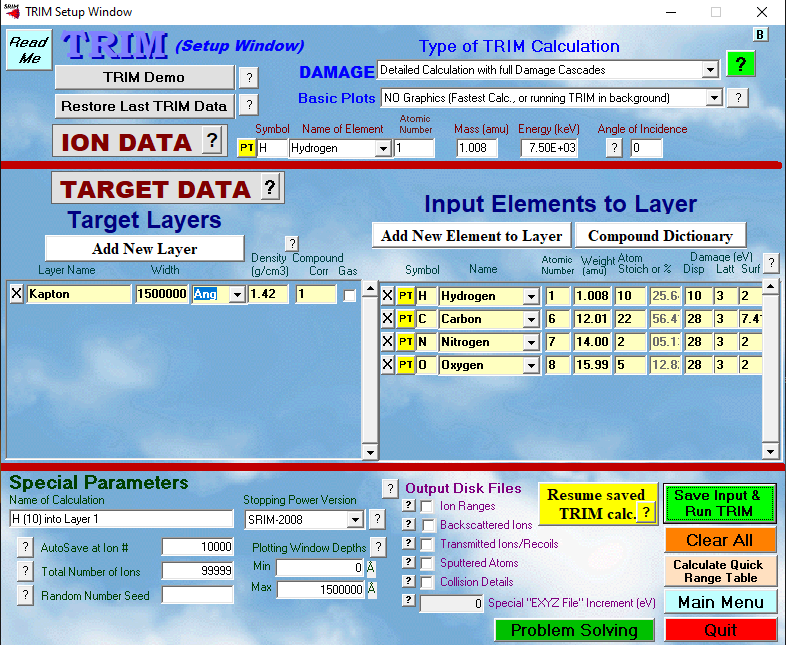
\includegraphics[width=1\textwidth]{../SRIM_setup.PNG}
	\caption{Example of TRIM setup.}\label{fig:SRIM_setup}
\end{figure}

The dose deposited in Kapton depends on the energy of the incident protons. As the energy increases, the depth of the deposited dose increases. In Figure \ref{fig:dose_depth_percentile_vs_energy}, the colored solid curves show the percentiles of dose deposited less than a particular depth, as a function of energy for normally incident protons. For example, the purple curve shows the depth vs.\ energy at which $95\%$ of the dose is deposited. From Figure~\ref{fig:dose_depth_percentile_vs_energy}, it is clear that the dose is not deposited  uniformly. Thicknesses between the green and blue curves, $45\%$ of the dose is deposited, as well as between the green and purple curves. Therefore, $90\%$ of the dose is deposited between the blue and purple curves. In general, the depth vs. energy profile has a double-power-law shape (depth in angstrom $\angstrom$ and energy in electron volts eV)
\begin{equation}\label{eq:double-power-law}
	D(E) = \left(\frac{E}{a}\right)^b + \left(\frac{E}{c}\right)^d,
\end{equation}
where $a$ is the low-energy scale, $c$ is the high-energy scale, and $b$ \& $d$ are the indices for each scale, respectively. As the percentile increases, the values for the energy scales $a$ and $c$ decreases. For a list of parameter fits, see Table \ref{tab:double-power-law-parameters} in Appendix \ref{App:Dose Percentile-Depth vs. Energy Parameters Fits}. Observing that $b < d$, the Kapton material is more effective at stopping lower energy protons ($ < \sim 100$ keV) than higher energy protons.

\begin{figure}[htbp!]
	\centering
	\includegraphics[width=0.95\textwidth]{../Bragg_peak_data/dose_depth_percentile_vs_energy.png}
	\caption{Left axis: Depth in Kapton vs.\ energy for various dose-depth percentiles. Right axis: Dose per fluence vs.\ energy.}\label{fig:dose_depth_percentile_vs_energy}
\end{figure}


The dotted-dashed curve in Figure \ref{fig:dose_depth_percentile_vs_energy} shows the total dose deposited per fluence as a function of energy. Basically, this curve can be thought of as the dose cross-section of Kapton for normally incident protons. One way to find the total dose for a given energy spectrum, one could convolute the dose cross-section with the differential energy spectrum, taking into account the depth percentile for a particular thickness of Kapton material. However, a more direct method to find the total dose is used in the following sections.

%%%%%%%%%%%%%%%%%%%%%%%%%%%%%%%%%%%%%%%%%%%%%%%%%%%%%%%%%%%%%%%%%%
%%%%%%%%%%%%%%%%%%%%%%%%%%%%%%%%%%%%%%%%%%%%%%%%%%%%%%%%%%%%%%%%%%
\section{Natural Environments}
\label{sec:Natural Environment}

The natural environments for the RCD of Solar Cruiser are separated into a mid-energy component (solar energetic particles, Section~\ref{ssec:natenv-Solar Particle Events}) and a low-energy component (background solar wind, Section~\ref{ssec:natenv-Low-Energy Solar Wind}). The high-energy component (galactic cosmic rays, $> \text{GeV}$) are omitted because of the thin materials studied in this analysis. In general, for an isotropic proton environment with energies greater than $\sim 13.1$~MeV (see Equation~\eqref{eq:E_5perc}), the particles do not deposit a significant amount of energy in $150 \mu$m Kapton (i.e., the Bragg peak has not been reached yet).


%%%%%%%%%%%%%%%%%%%%%%%%%%%%%%%%%%%%%%%%%%%%%%%%%%%%%%%%%%%%%%%%%%
%%%%%%%%%%%%%%%%%%%%%%%%%%%%%%%%%%%%%%%%%%%%%%%%%%%%%%%%%%%%%%%%%%
\subsection{Solar Particle Events}
\label{ssec:natenv-Solar Particle Events}

The solar particle event (SPE) environment for interplanetary space is derived following the same procedure as outlined in the Cross-Program Design Specification for Natural Environments (DSNE) Section 3.3.1 (see the technical notes at the end of the section). A 2-year trajectory is defined in interplanetary space at the sub-L1 location of 0.984 AU in SPENVIS\footnote{\url{https://www.spenvis.oma.be/}} under the \textsf{Coordinate generators} tab. Once this is set, the SPE fluence is computed under the \textsf{Solar particle mission fluences}. The following parameters are set:
\begin{itemize}
	\item Solar particle model: ESP-PSYCHIC (total fluence)
	\item Ion range: H to H
	\item Prediction period: override
	\item Prediction period [years]: 2.0
	\item Offset in solar cycle: override
	\item Offset from solar maximum [years]: 0
	\item Confidence level [\%]: 95.0
\end{itemize}

Note that the \textsf{total fluence} mode is used rather than the \textsf{worst event fluence} mode. In DSNE, the 1-year unshielded SPE (Table 3.3.1.10.2-1) uses the \textsf{worst event fluence} mode. However, for mission length longer than a year, the \textsf{total fluence} mode should be used. For example, the 15-year unshielded SPE TID environment (Table 3.3.1.10.2-5) uses the proton environment from ESP-PSYCHIC using the \textsf{total fluence} mode.

Table \ref{tab:ESP-PSYCHIC_2-year_subL1} shows the down-selected energy bins that match DSNE Table 3.3.1.10.2-1. In terms of fluence $> 100$ keV, the 2-year SPE environment shown in Table \ref{tab:ESP-PSYCHIC_2-year_subL1} is $3.7\times$ greater than the unshielded SPE environment is DSNE Table 3.3.1.10.2-1.%, despite the fluence duration doubling.
This is why it is important to run the ESP-PSYCHIC model for the required mission length and not multiply Table 3.3.1.10.2-1 by the number of years.% Otherwise, a large overestimate occurs. 

\begin{table}[!h]\centering
	\caption{ESP-PSYCHIC total fluence of protons for 2 years during solar maximum at 0.984 AU. The energy center $=\sqrt{\text{bin left edge}\times\text{bin right edge}.}$ }\label{tab:ESP-PSYCHIC_2-year_subL1}
	\begin{tabular}{|c | c | c | c |}\hline
		Energy Center (keV) & Bin Flux (\#/cm$^2$) & Bin Width (keV) & Bin Left Edge (keV) \\\hline

1.58E+02&8.04E+11&1.50E+02&1.00E+02\\\hline
3.54E+02&3.62E+11&2.50E+02&2.50E+02\\\hline
7.07E+02&2.33E+11&5.00E+02&5.00E+02\\\hline
1.41E+03&1.50E+11&1.00E+03&1.00E+03\\\hline
2.65E+03&8.57E+10&1.50E+03&2.00E+03\\\hline
4.18E+03&4.59E+10&1.50E+03&3.50E+03\\\hline
5.96E+03&3.85E+10&2.10E+03&5.00E+03\\\hline
7.54E+03&1.16E+10&9.00E+02&7.10E+03\\\hline
8.49E+03&1.02E+10&1.00E+03&8.00E+03\\\hline
9.49E+03&8.09E+09&1.00E+03&9.00E+03\\\hline
1.26E+04&3.02E+10&6.00E+03&1.00E+04\\\hline
1.70E+04&5.77E+09&2.00E+03&1.60E+04\\\hline
1.90E+04&4.45E+09&2.00E+03&1.80E+04\\\hline
2.24E+04&8.14E+09&5.00E+03&2.00E+04\\\hline
2.96E+04&8.87E+09&1.00E+04&2.50E+04\\\hline
3.74E+04&2.56E+09&5.00E+03&3.50E+04\\\hline
4.24E+04&1.90E+09&5.00E+03&4.00E+04\\\hline
4.74E+04&1.43E+09&5.00E+03&4.50E+04\\\hline
5.96E+04&3.36E+09&2.10E+04&5.00E+04\\\hline
7.54E+04&7.50E+08&9.00E+03&7.10E+04\\\hline
8.49E+04&5.95E+08&1.00E+04&8.00E+04\\\hline
9.49E+04&4.28E+08&1.00E+04&9.00E+04\\\hline
1.26E+05&1.05E+09&6.00E+04&1.00E+05\\\hline
1.70E+05&1.32E+08&2.00E+04&1.60E+05\\\hline
1.90E+05&9.10E+07&2.00E+04&1.80E+05\\\hline
2.24E+05&1.32E+08&5.00E+04&2.00E+05\\\hline
3.16E+05&1.23E+08&1.50E+05&2.50E+05\\\hline
4.47E+05&2.12E+07&1.00E+05&4.00E+05\\\hline
	\end{tabular}
\end{table}
\clearpage % forces the figure to drop before this point

%%%%%%%%%%%%%%%%%%%%%%%%%%%%%%%%%%%%%%%%%%%%%%%%%%%%%%%%%%%%%%%%%%
%%%%%%%%%%%%%%%%%%%%%%%%%%%%%%%%%%%%%%%%%%%%%%%%%%%%%%%%%%%%%%%%%%
\subsection{Low-Energy Solar Wind}
\label{ssec:natenv-Low-Energy Solar Wind}

To compute the low-energy solar wind plasma contribution of the environment (assumed at 1 AU), the L2-CPE V1.3 software package was used. The proton fluence was computed with the setup shown in Figure \ref{fig:L2-CPE-Setup}. Other percentiles that are automatically calculated are $5\%$, $50\%$, $95\%$, and the maximum, mean, and minimum fluxes for each energy bin (see Listing \ref{lst:FLX_PTNXPOS_SWMX_IMP} in Appendix \ref{App:Raw L2-CPE output of the Interplanetary Proton Environment}). Table \ref{tab:p95_sunward_solarwind_IMP} shows the reduced data in the same format as Table \ref{tab:ESP-PSYCHIC_2-year_subL1}. The $95\%$ is used in accordance with DSNE (see the technical notes at the end of Section 3.3.1). The sunward facing flux is used and assumed to be isotropic as worst-case. 

\begin{figure}[htbp!]
	\centering
	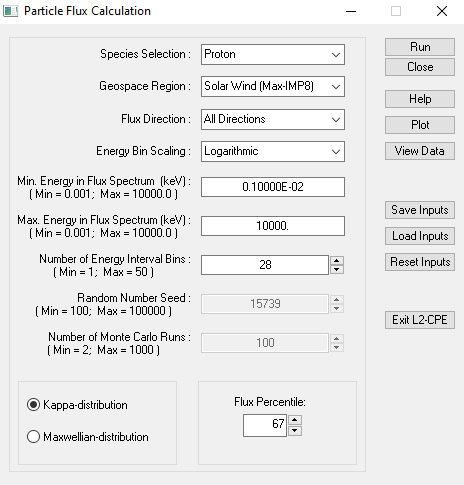
\includegraphics[width=0.75\textwidth]{../L2CPE/L2-CPE-Setup.PNG}
	\caption{Screen shot of the setup used in computing the low-energy proton flux environment in L2-CPE.}\label{fig:L2-CPE-Setup}
\end{figure}




\begin{table}[!h]\centering
	\caption{The $95\%$ sunward solar wind environment from L2-CPE for 2 years. The energy center $=\sqrt{\text{bin left edge}\times\text{bin right edge}.}$}\label{tab:p95_sunward_solarwind_IMP}
	\begin{tabular}{|c | c | c | c |}\hline
		Energy Center (keV) & Bin Flux (\#/cm$^2$) & Bin Width (keV) & Bin Left Edge (keV) \\\hline
1.34E-03&4.97E+09&8.00E-04&1.00E-03\\\hline
2.40E-03&8.36E+09&1.40E-03&1.80E-03\\\hline
4.23E-03&1.38E+10&2.40E-03&3.20E-03\\\hline
7.48E-03&2.24E+10&4.40E-03&5.60E-03\\\hline
1.33E-02&3.50E+10&7.80E-03&1.00E-02\\\hline
2.37E-02&5.29E+10&1.38E-02&1.78E-02\\\hline
4.21E-02&7.66E+10&2.46E-02&3.16E-02\\\hline
7.50E-02&1.05E+11&4.38E-02&5.62E-02\\\hline
1.33E-01&1.37E+11&7.78E-02&1.00E-01\\\hline
2.37E-01&1.64E+11&1.38E-01&1.78E-01\\\hline
4.22E-01&1.86E+11&2.46E-01&3.16E-01\\\hline
7.50E-01&1.94E+11&4.38E-01&5.62E-01\\\hline
1.33E+00&1.88E+11&7.78E-01&1.00E+00\\\hline
2.37E+00&1.68E+11&1.38E+00&1.78E+00\\\hline
4.22E+00&1.40E+11&2.46E+00&3.16E+00\\\hline
7.50E+00&1.10E+11&4.38E+00&5.62E+00\\\hline
1.33E+01&8.21E+10&7.78E+00&1.00E+01\\\hline
2.37E+01&5.75E+10&1.38E+01&1.78E+01\\\hline
4.22E+01&3.91E+10&2.46E+01&3.16E+01\\\hline
7.50E+01&2.56E+10&4.38E+01&5.62E+01\\\hline
1.33E+02&1.65E+10&7.78E+01&1.00E+02\\\hline
2.37E+02&1.04E+10&1.38E+02&1.78E+02\\\hline
4.22E+02&6.43E+09&2.46E+02&3.16E+02\\\hline
7.50E+02&3.91E+09&4.38E+02&5.62E+02\\\hline
1.33E+03&2.35E+09&7.78E+02&1.00E+03\\\hline
2.37E+03&1.43E+09&1.38E+03&1.78E+03\\\hline
4.22E+03&8.50E+08&2.46E+03&3.16E+03\\\hline
7.50E+03&5.05E+08&4.38E+03&5.62E+03\\\hline
	\end{tabular}
\end{table}
\clearpage % forces the figure to drop before this point

%%%%%%%%%%%%%%%%%%%%%%%%%%%%%%%%%%%%%%%%%%%%%%%%%%%%%%%%%%%%%%%%%%
%%%%%%%%%%%%%%%%%%%%%%%%%%%%%%%%%%%%%%%%%%%%%%%%%%%%%%%%%%%%%%%%%%
\section{Total Ionizing Dose}

The Stopping and Range of Ions in Matter (SRIM) is a group of programs that calculate the stopping and range of ions in matter\footnote{\url{http://www.srim.org/SRIM/SRIMINTRO.htm}}. % The ion stopping and range table calculator in SRIM was used in Section \ref{sssec:ProtonStoppingDistance}.
For each run using TRIM (Transport of Ions in Matter), a mono-energetic beam of a single incident angle is used at the environment and transported through a series of predefined layers in a Monte Carlo fashion.

The isotropic flux for a particular energy and incident angle $\Phi(E,\theta)$ can be computed as (using a cosine distribution for an incident isotropic distribution on a flat slab)
\begin{align}
	\Phi(E,\theta) &= [\Phi(E_i) - \Phi(E_{i+1})] \frac{\cos(2\theta_i) - \cos(2\theta_{i+1})}{2},\nonumber\\
	&= [\Phi(E_i) - \Phi(E_{i+1})] w_i,
\end{align}
where $E = \sqrt{E_i E_{i+1}}$, $\theta = (\theta_i + \theta_{i+1})/2$, and $\Phi(E_i)$ is the integral flux at energy $E_i$ (e.g., Section \ref{sec:Natural Environment}). The TRIM simulation is run using $E$ and $\theta$ as centered values in the energy-angle bin. The angular weight term follows from the integral
\begin{equation}
	w_i = 2\int_{\theta_i}^{\theta_{i+1}}d\theta\sin\theta\cos\theta = \frac{\cos(2\theta_i) - \cos(2\theta_{i+1})}{2},
\end{equation}
where it is assumed that the incident angle $\theta$ ranges\footnote{Initially, the range of the incident angle is from $-90^\circ$ to $90^\circ$, but it is assumed the dose profiles will be symmetric about $0^\circ$.} from $0^\circ$ to $90^\circ$, hence the factor of $2$. In this analysis, the range of incident angles $\theta$ are given in Table \ref{tab:incidentAngleBins}.

\begin{table}[h]\centering
	\caption{Angular weight factors $w_i$ where $\sum_i w_i = 1$. The $\theta_i$ and $\theta_{i+1}$ are bin edges where $\theta$ is taken as the approximate bin center.}\label{tab:incidentAngleBins}
	\begin{tabular}{|c | c | c | c | c |}\hline
		index $i$ & $\theta_i$ & $\theta_{i+1}$ & $\theta$ & $w_i$ \\\hline
		0  & 0.00 & 15.0 & 0.00 & 3.40E-2 \\\hline
		1  & 15.0 & 37.5 & 30.0 & 1.73E-1 \\\hline
		2  & 37.5 & 52.5 & 45.0 & 1.85E-1\\\hline
		3  & 52.5 & 67.5 & 60.0 & 2.26E-1 \\\hline
		4  & 67.5 & 82.5 & 75.0 & 2.52E-1\\\hline
		5  & 82.5 & 90.0 & 87.0 & 1.30E-1\\\hline
	\end{tabular}
\end{table}

TID can be computed by saving the ionization file once a sufficient number of test particles are run. The ionization file contains information about the deposited ionization energy due to the primary ions $D_{\text{ions}}$ and to secondaries $D_{\text{recoils}}$ (called recoils) as a function of target depth. The ionization energy units are in eV per Angstrom per ion. To convert the deposited energy into rads, as a function of incident ion energy, angle and deposited depth, the following conversion equation is used
\begin{equation}
	D(E,\theta,r) = [D_{\text{ions}} + D_{\text{recoils}}](E,\theta,r) \times \frac{10^8 \text{ \si{\angstrom}}}{\text{cm}} \times \frac{1.60218\times 10^{-19} \text{ J}}{\text{eV}} \times \frac{\Phi(E,\theta)}{\rho[\text{kg cm$^{-3}$}]} ,
\end{equation}
where $\rho$ is the material density in units of kg cm$^{-3}$.

In Sections \ref{ssec:TID-Solar Particle Events} and \ref{ssec:TID-Low-Energy Solar Wind}, the dose vs.\ depth and dose vs.\ energy curves are discussed for the solar particle events and low-energy solar wind, respectively. Note that the \textit{rough} nature of the differential dose vs.\ depth curves found in Figures \ref{fig:ESP-PSYCHIC_totalfluence_2-year_subL1_Differential_Dose_vs_Depth} and \ref{fig:L2-CPE_2-year_95-percentile_Differential_Dose_vs_Depth} are due to the finite number of incident energies and angles probed. Since the poorly resolved portion occurs at lower doses, the overall estimated TID should be numerically stable.

The integral dose vs.\ depth curves shown in Figures \ref{fig:ESP-PSYCHIC_totalfluence_2-year_subL1_Integral_Dose_vs_Depth} and \ref{fig:L2-CPE_2-year_95-percentile_Integral_Dose_vs_Depth} can be interpreted as the dose deposited up to a particular depth (i.e., at that depth $d$ or less than $d$ towards the front facing surface).

In terms of energy, the integral dose vs. energy curves displayed in Figures \ref{fig:ESP-PSYCHIC_totalfluence_2-year_subL1_Integral_Dose_vs_Energy} and \ref{fig:L2-CPE_2-year_95-percentile_Integral_Dose_vs_Energy} show the TID from particles incident with a particular energy $E$ or greater. Since an isotropic flux environment is simulated, a clear break in the energy spectrum is not exactly seen. However, it is clear from the differential dose vs.\ energy plots (Figures \ref{fig:ESP-PSYCHIC_totalfluence_2-year_subL1_Differential_Dose_vs_Energy} and \ref{fig:L2-CPE_2-year_95-percentile_Differential_Dose_vs_Energy}) that the slope starts to fall off at around $E_{\text{crit}}=4$ MeV. This value of  $E_{\text{crit}}$ makes sense, because for $150 \mu$m of Kapton at the $99$ percentile of dose deposited, the corresponding energy is about $3.7$ MeV. That is, using the fit parameters from Table \ref{tab:double-power-law-parameters} for the $99$ percentile, omitting the low-energy terms ($a$ and $b$), the energy can be solved as
\begin{equation}
	E_{99\% \text{ dose}} = 1.393 \text{ keV} (D/ 1 \angstrom)^{0.554},
\end{equation}
where $D$ is the thickness of the material (valid for $1 \mu$m $< D < 1$m) and $E$ is the critical energy. For the upper limit of incident energy to depot less than $5\%$ of the total dose, the following equation can be used
\begin{equation}\label{eq:E_5perc}
	E_{5\% \text{ dose}} = 4.543 \text{ keV} (D/ 1 \angstrom)^{0.560},
\end{equation}
giving $E_{5\% \text{ dose}} = 13.1$ MeV for $D = 150\mu$m.


%%%%%%%%%%%%%%%%%%%%%%%%%%%%%%%%%%%%%%%%%%%%%%%%%%%%%%%%%%%%%%%%%%
%%%%%%%%%%%%%%%%%%%%%%%%%%%%%%%%%%%%%%%%%%%%%%%%%%%%%%%%%%%%%%%%%%
\subsection{Solar Particle Events}
\label{ssec:TID-Solar Particle Events}

The solar particle event (SPE) environment (from ESP-PSYCHIC) used in computing the total ionizing dose (TID) to $150 \mu$m of Kapton can be found in Table \ref{tab:ESP-PSYCHIC_2-year_subL1} (Section \ref{ssec:natenv-Solar Particle Events}).  Dose vs.\ depth is covered in Section \ref{sssec:TID-SPE-Dose vs Depth} and Dose vs.\ energy in Section \ref{sssec:TID-SPE-Dose vs Energy}.

\newpage
\subsubsection{Total Ionizing Dose vs.\ Material Depth}
\label{sssec:TID-SPE-Dose vs Depth}

\begin{figure}[htbp!]
	\centering
	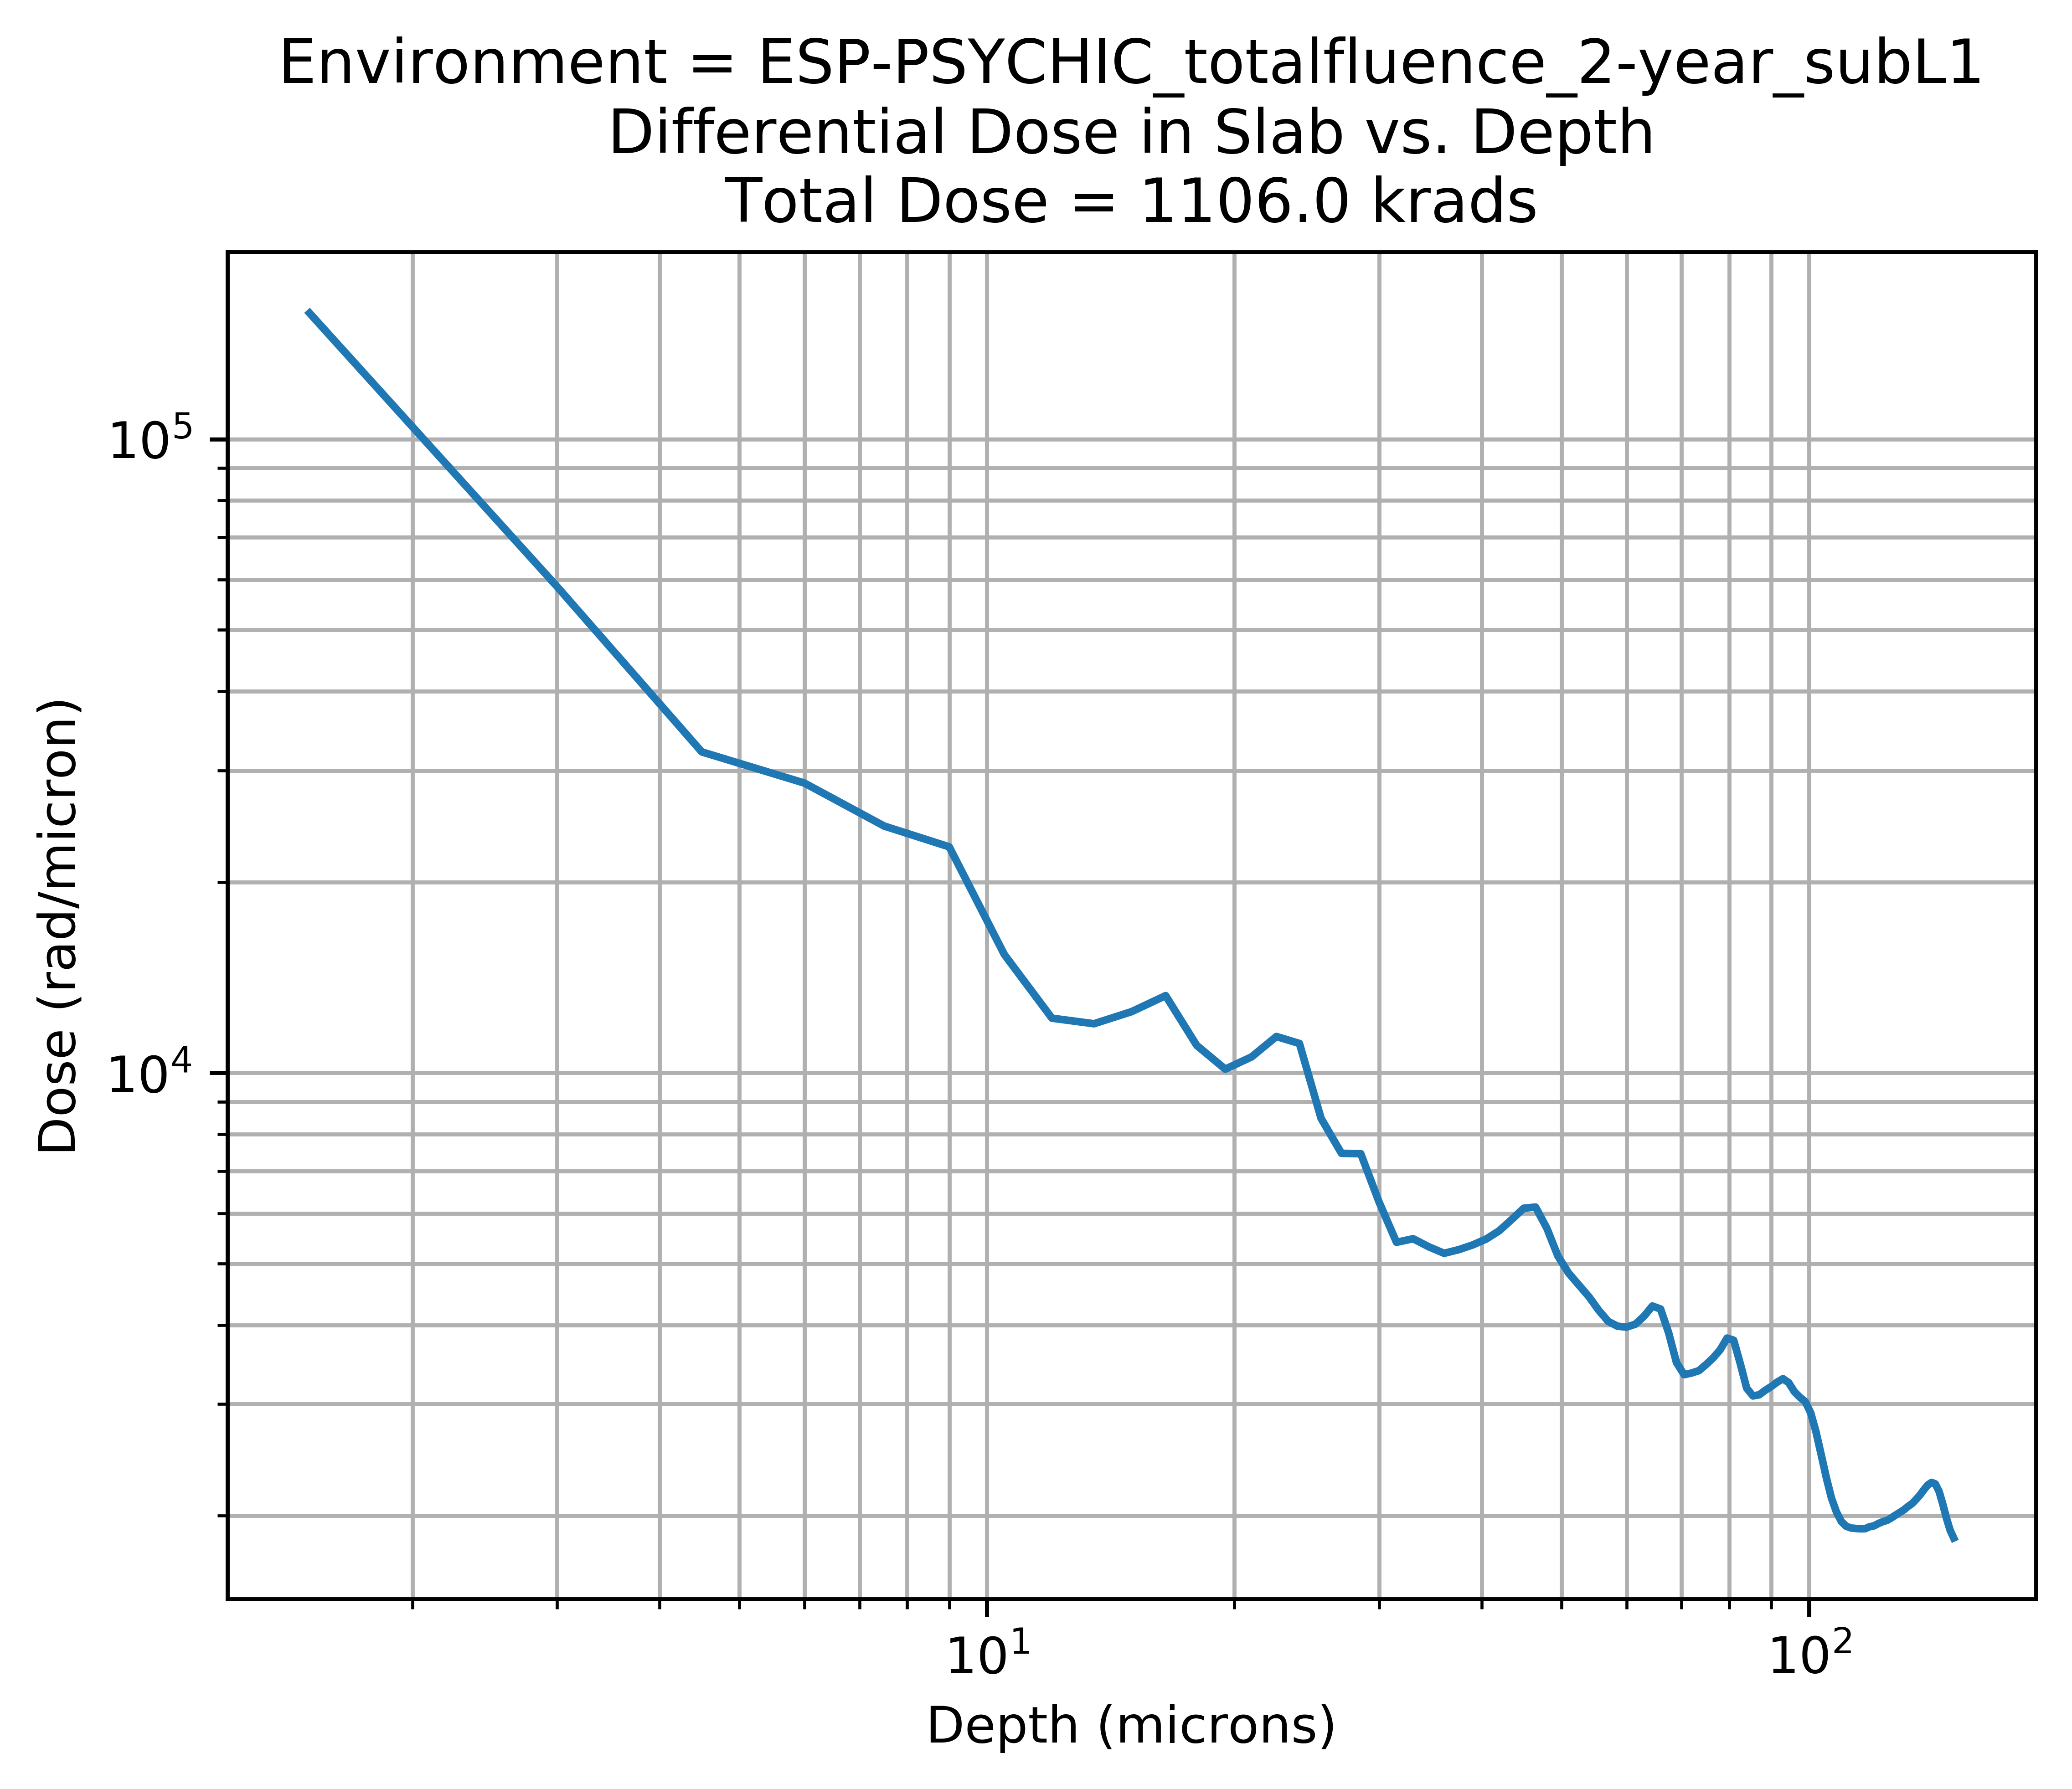
\includegraphics[width=0.95\textwidth]{../ESP-PSYCHIC_totalfluence_2-year_subL1_Differential_Dose_vs_Depth.png}
	\caption{The differential TID vs.\ depth for a 2-year isotropic SPE environment at 0.984 AU in $150 \mu$m of Kapton.}\label{fig:ESP-PSYCHIC_totalfluence_2-year_subL1_Differential_Dose_vs_Depth}
\end{figure}

\begin{figure}[htbp!]
	\centering
	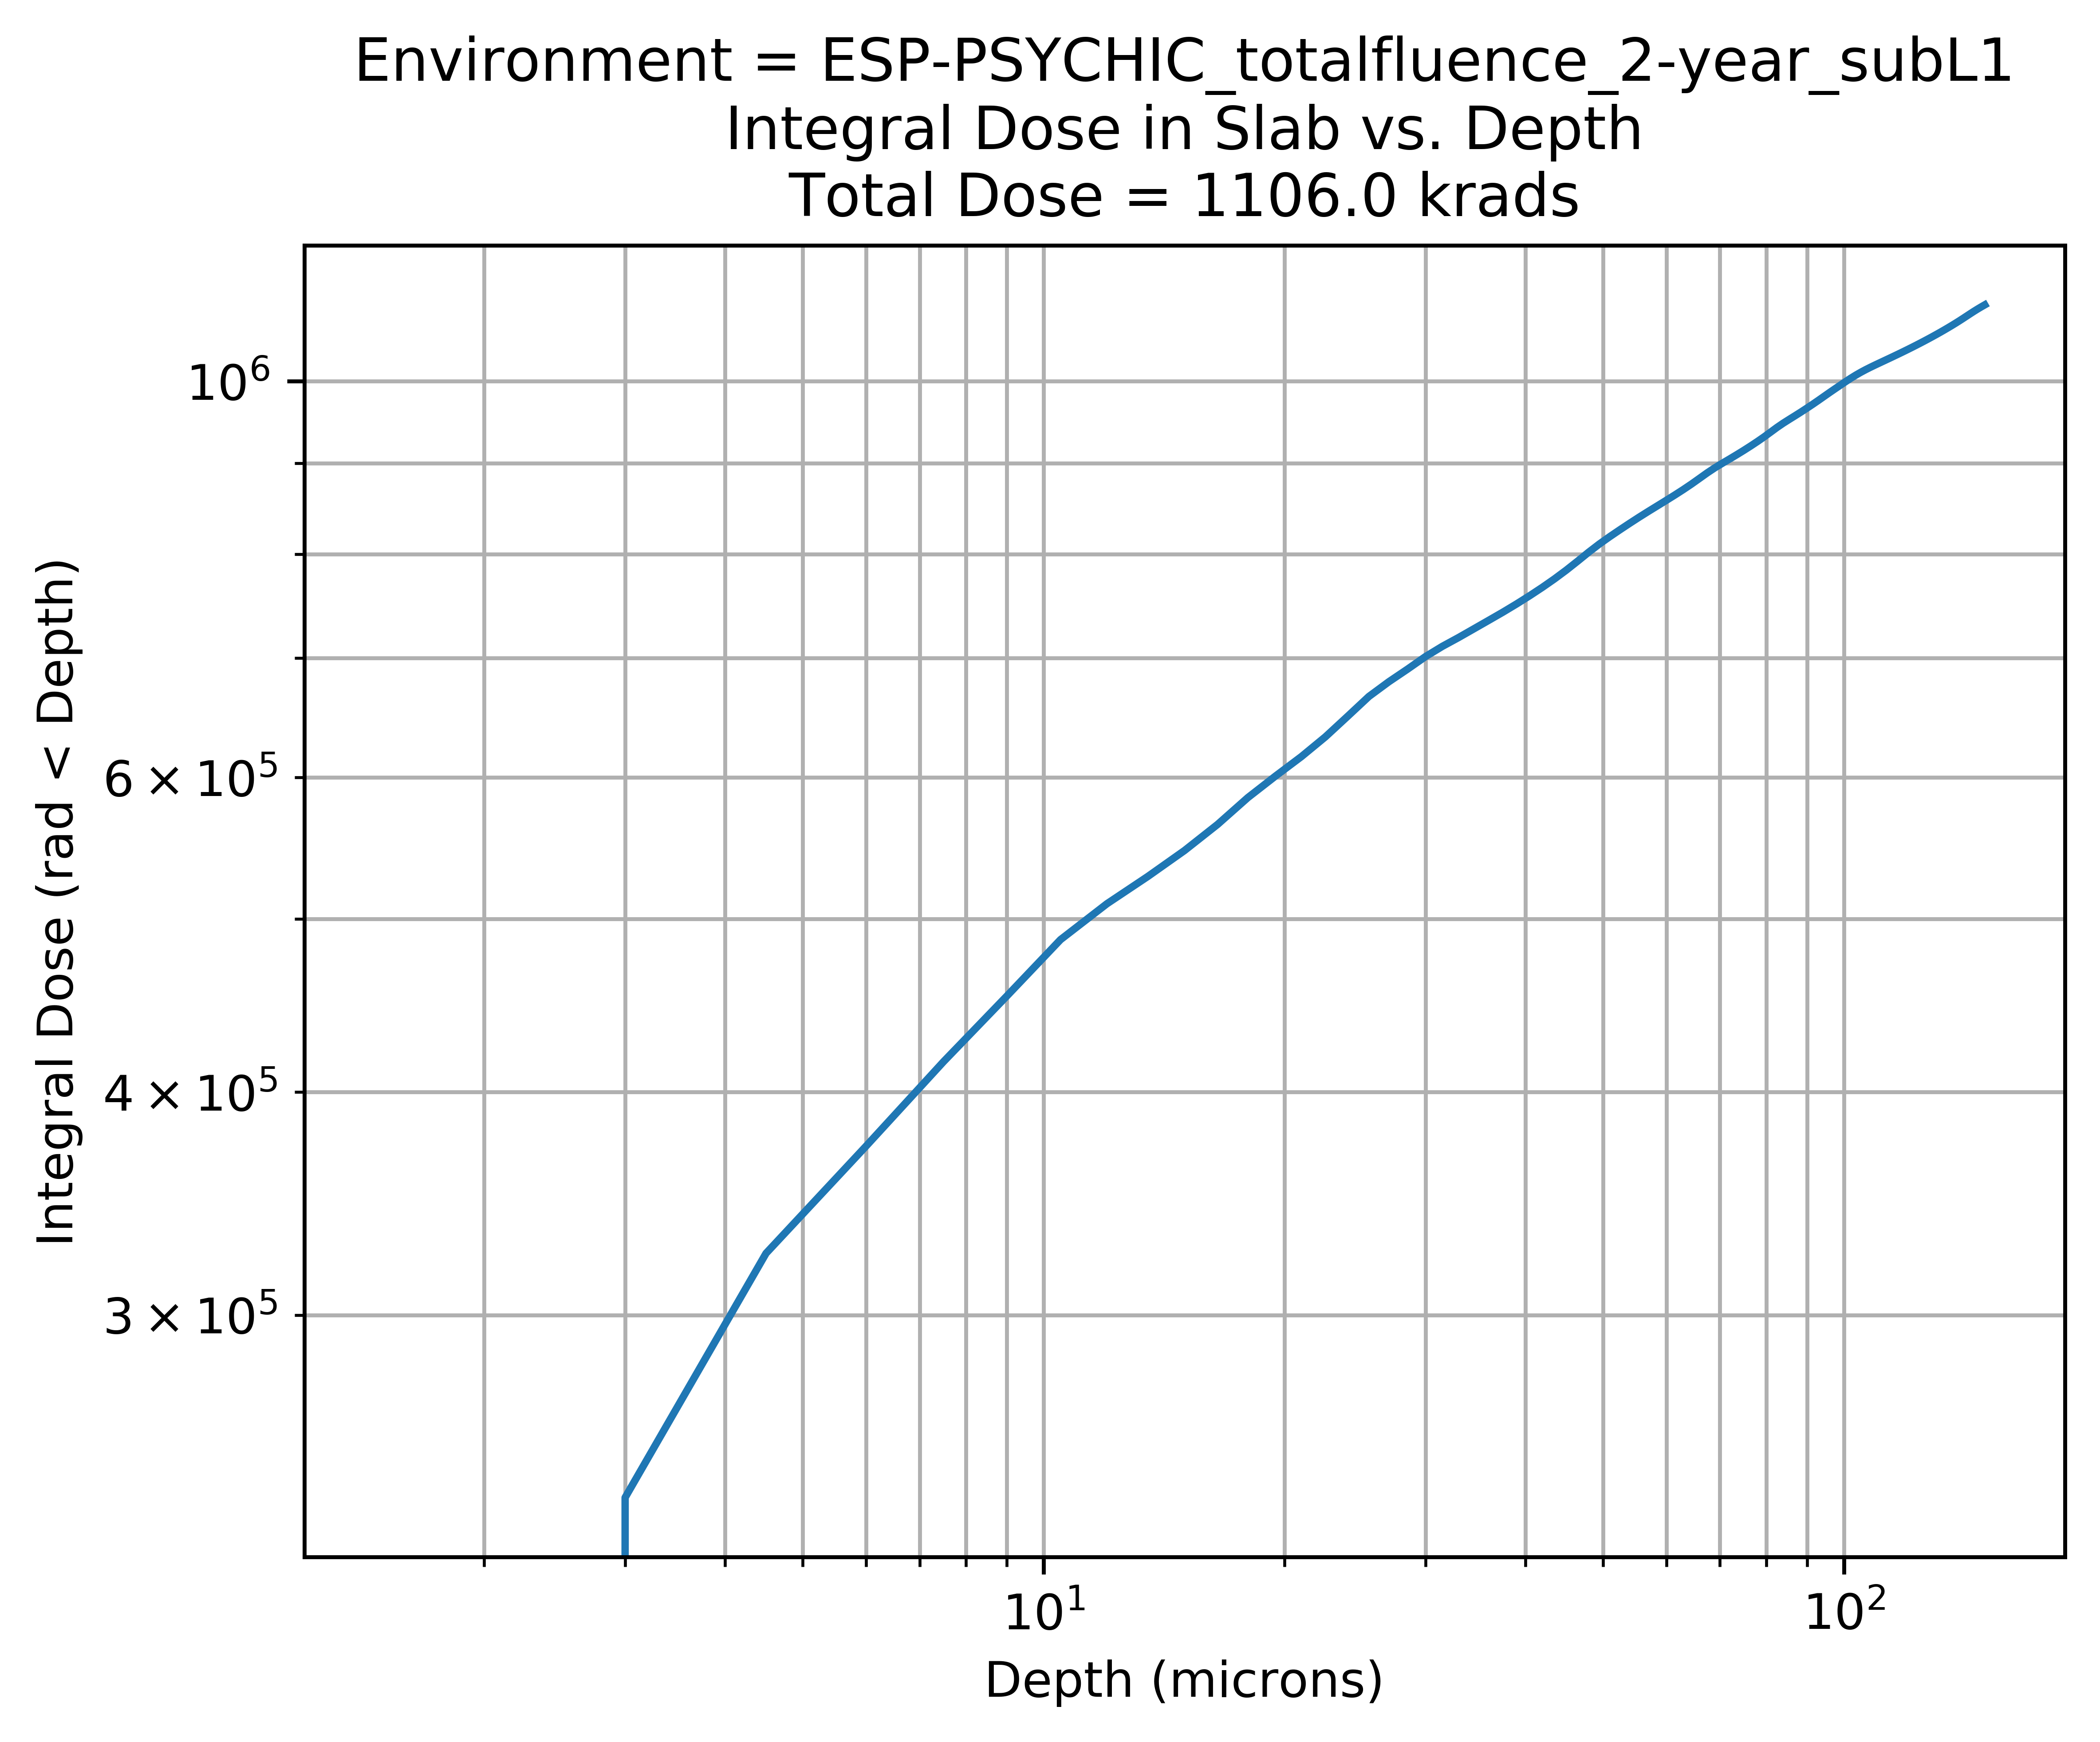
\includegraphics[width=0.95\textwidth]{../ESP-PSYCHIC_totalfluence_2-year_subL1_Integral_Dose_vs_Depth.png}
	\caption{The integral TID (less than a certain depth) vs.\ depth for a 2-year isotropic SPE environment at 0.984 AU in $150 \mu$m of Kapton.}\label{fig:ESP-PSYCHIC_totalfluence_2-year_subL1_Integral_Dose_vs_Depth}
\end{figure}

\clearpage % forces the figure to drop before this point

\subsubsection{Total Ionizing Dose vs.\ Proton Energy}
\label{sssec:TID-SPE-Dose vs Energy}

\begin{figure}[htbp!]
	\centering
	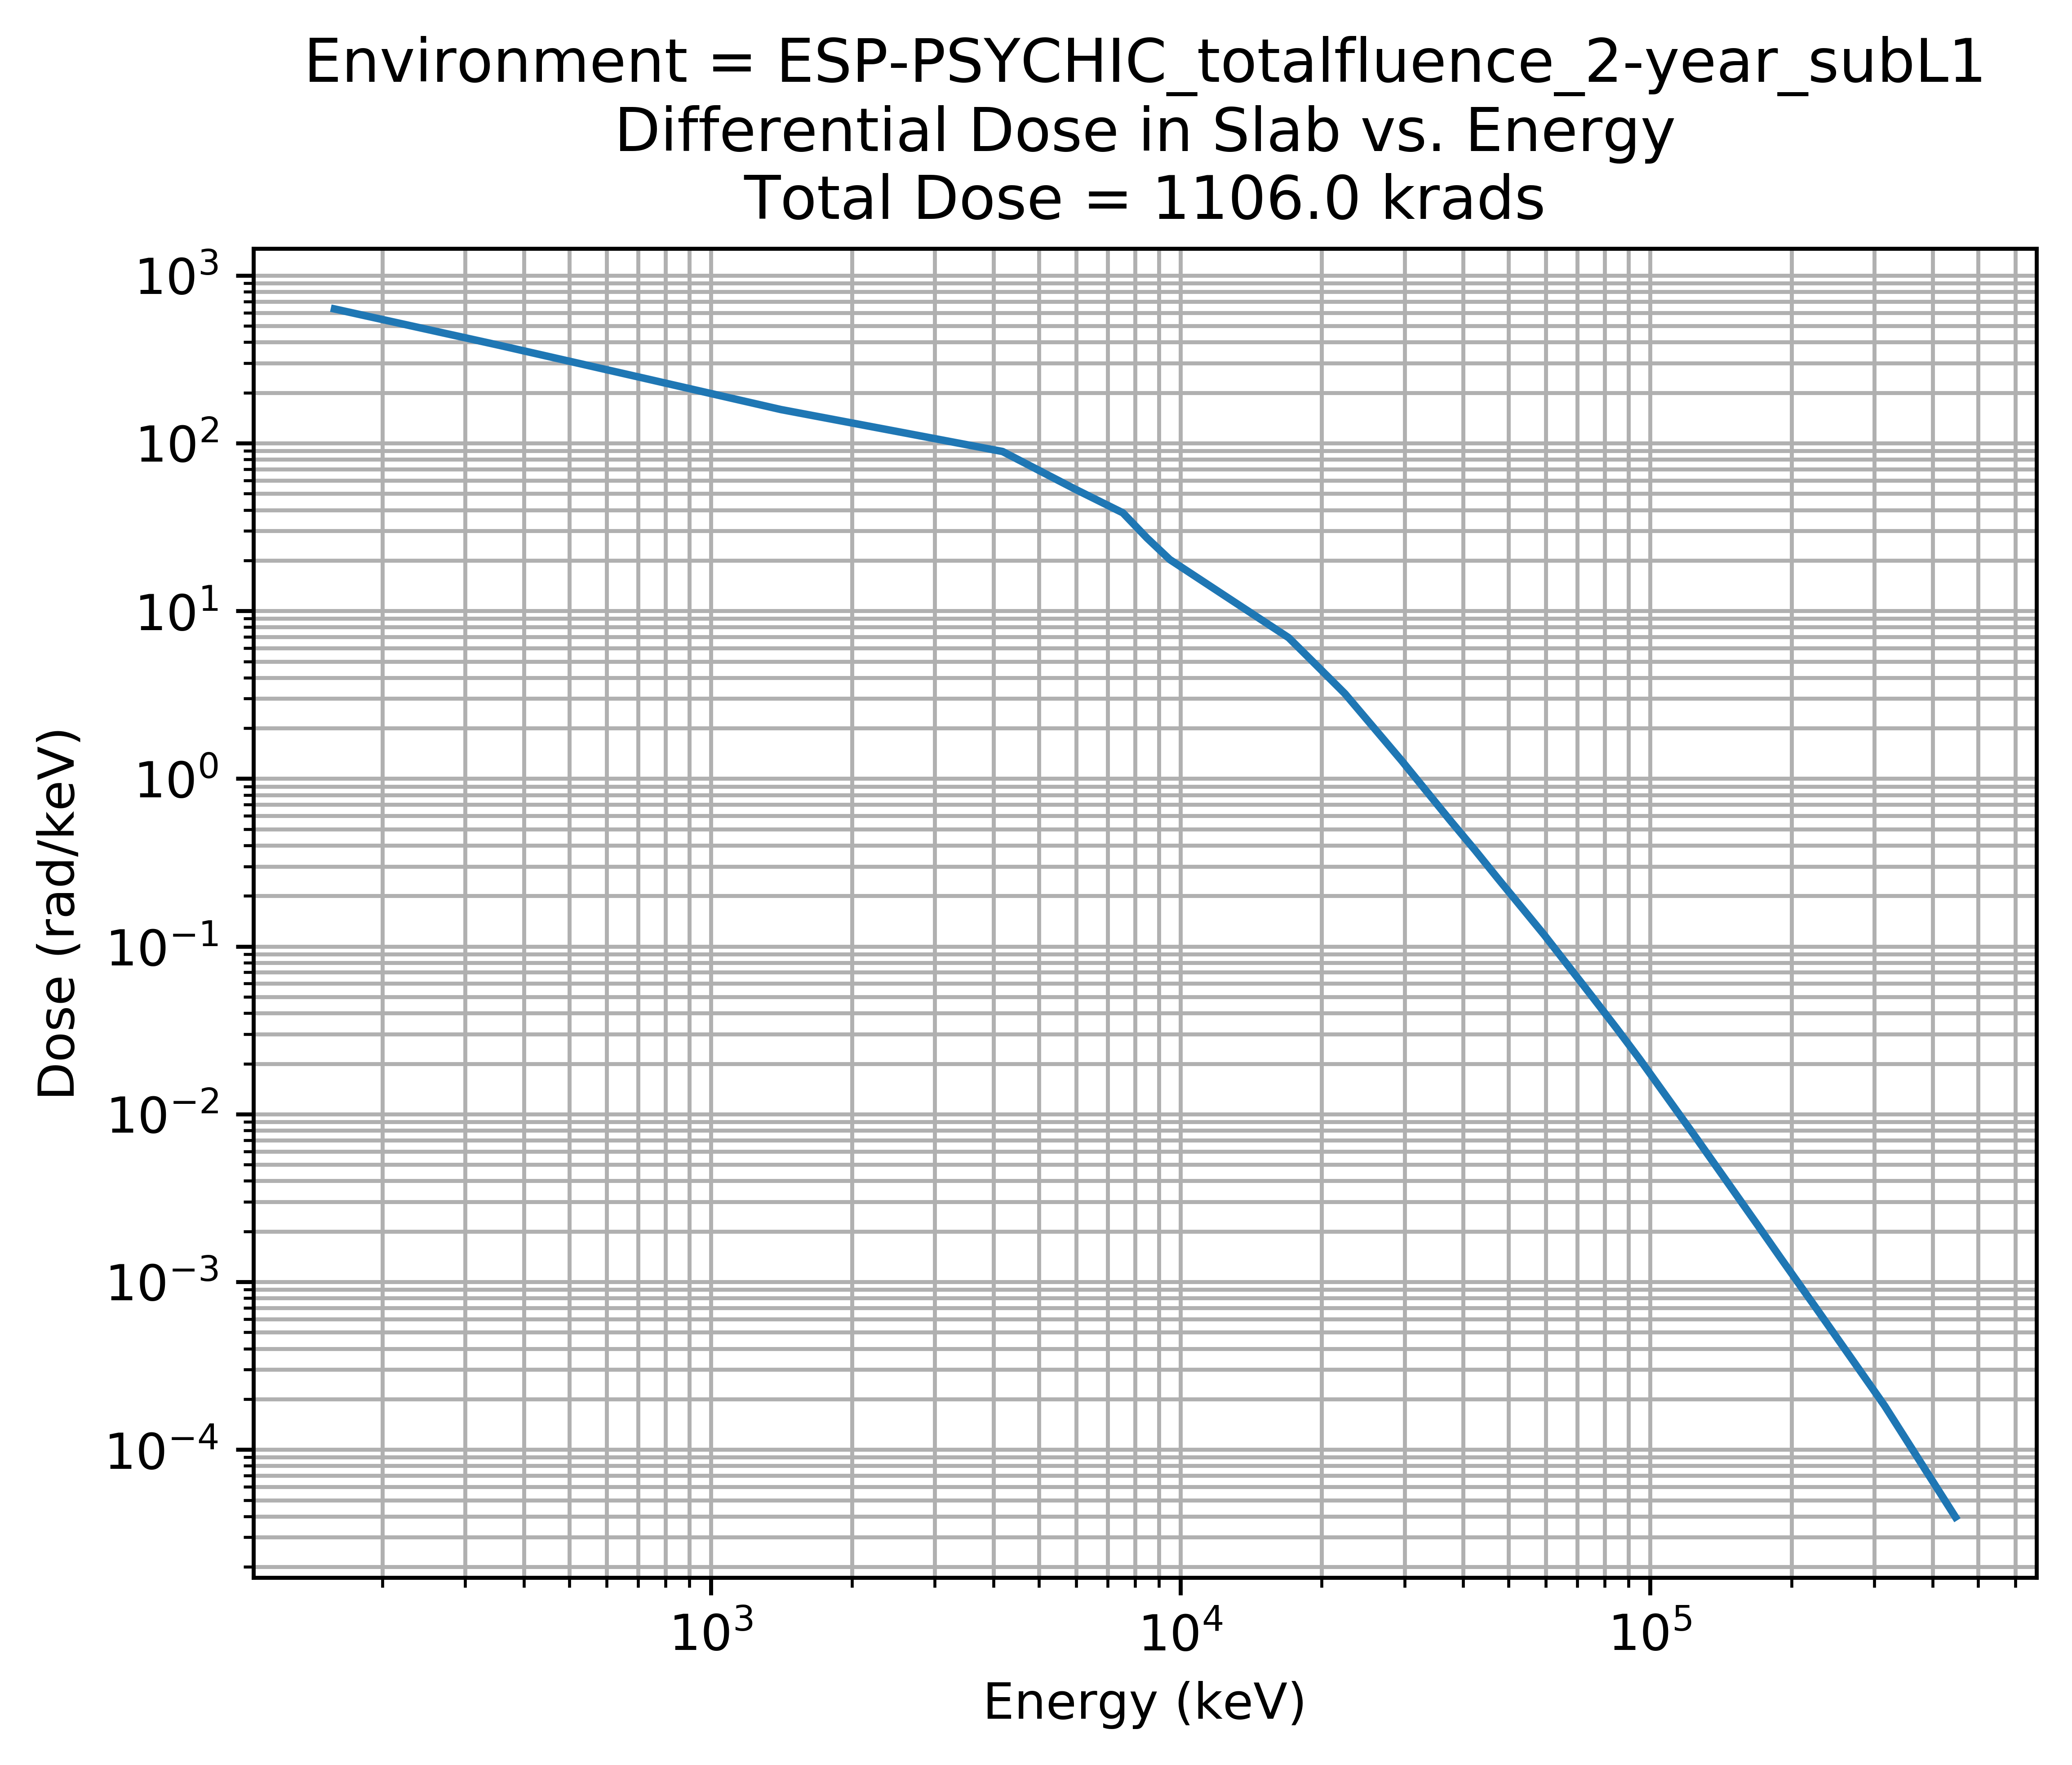
\includegraphics[width=0.95\textwidth]{../ESP-PSYCHIC_totalfluence_2-year_subL1_Differential_Dose_vs_Energy.png}
	\caption{The differential TID vs.\ energy for a 2-year isotropic SPE environment at 0.984 AU in $150 \mu$m of Kapton.}\label{fig:ESP-PSYCHIC_totalfluence_2-year_subL1_Differential_Dose_vs_Energy}
\end{figure}

\begin{figure}[htbp!]
	\centering
	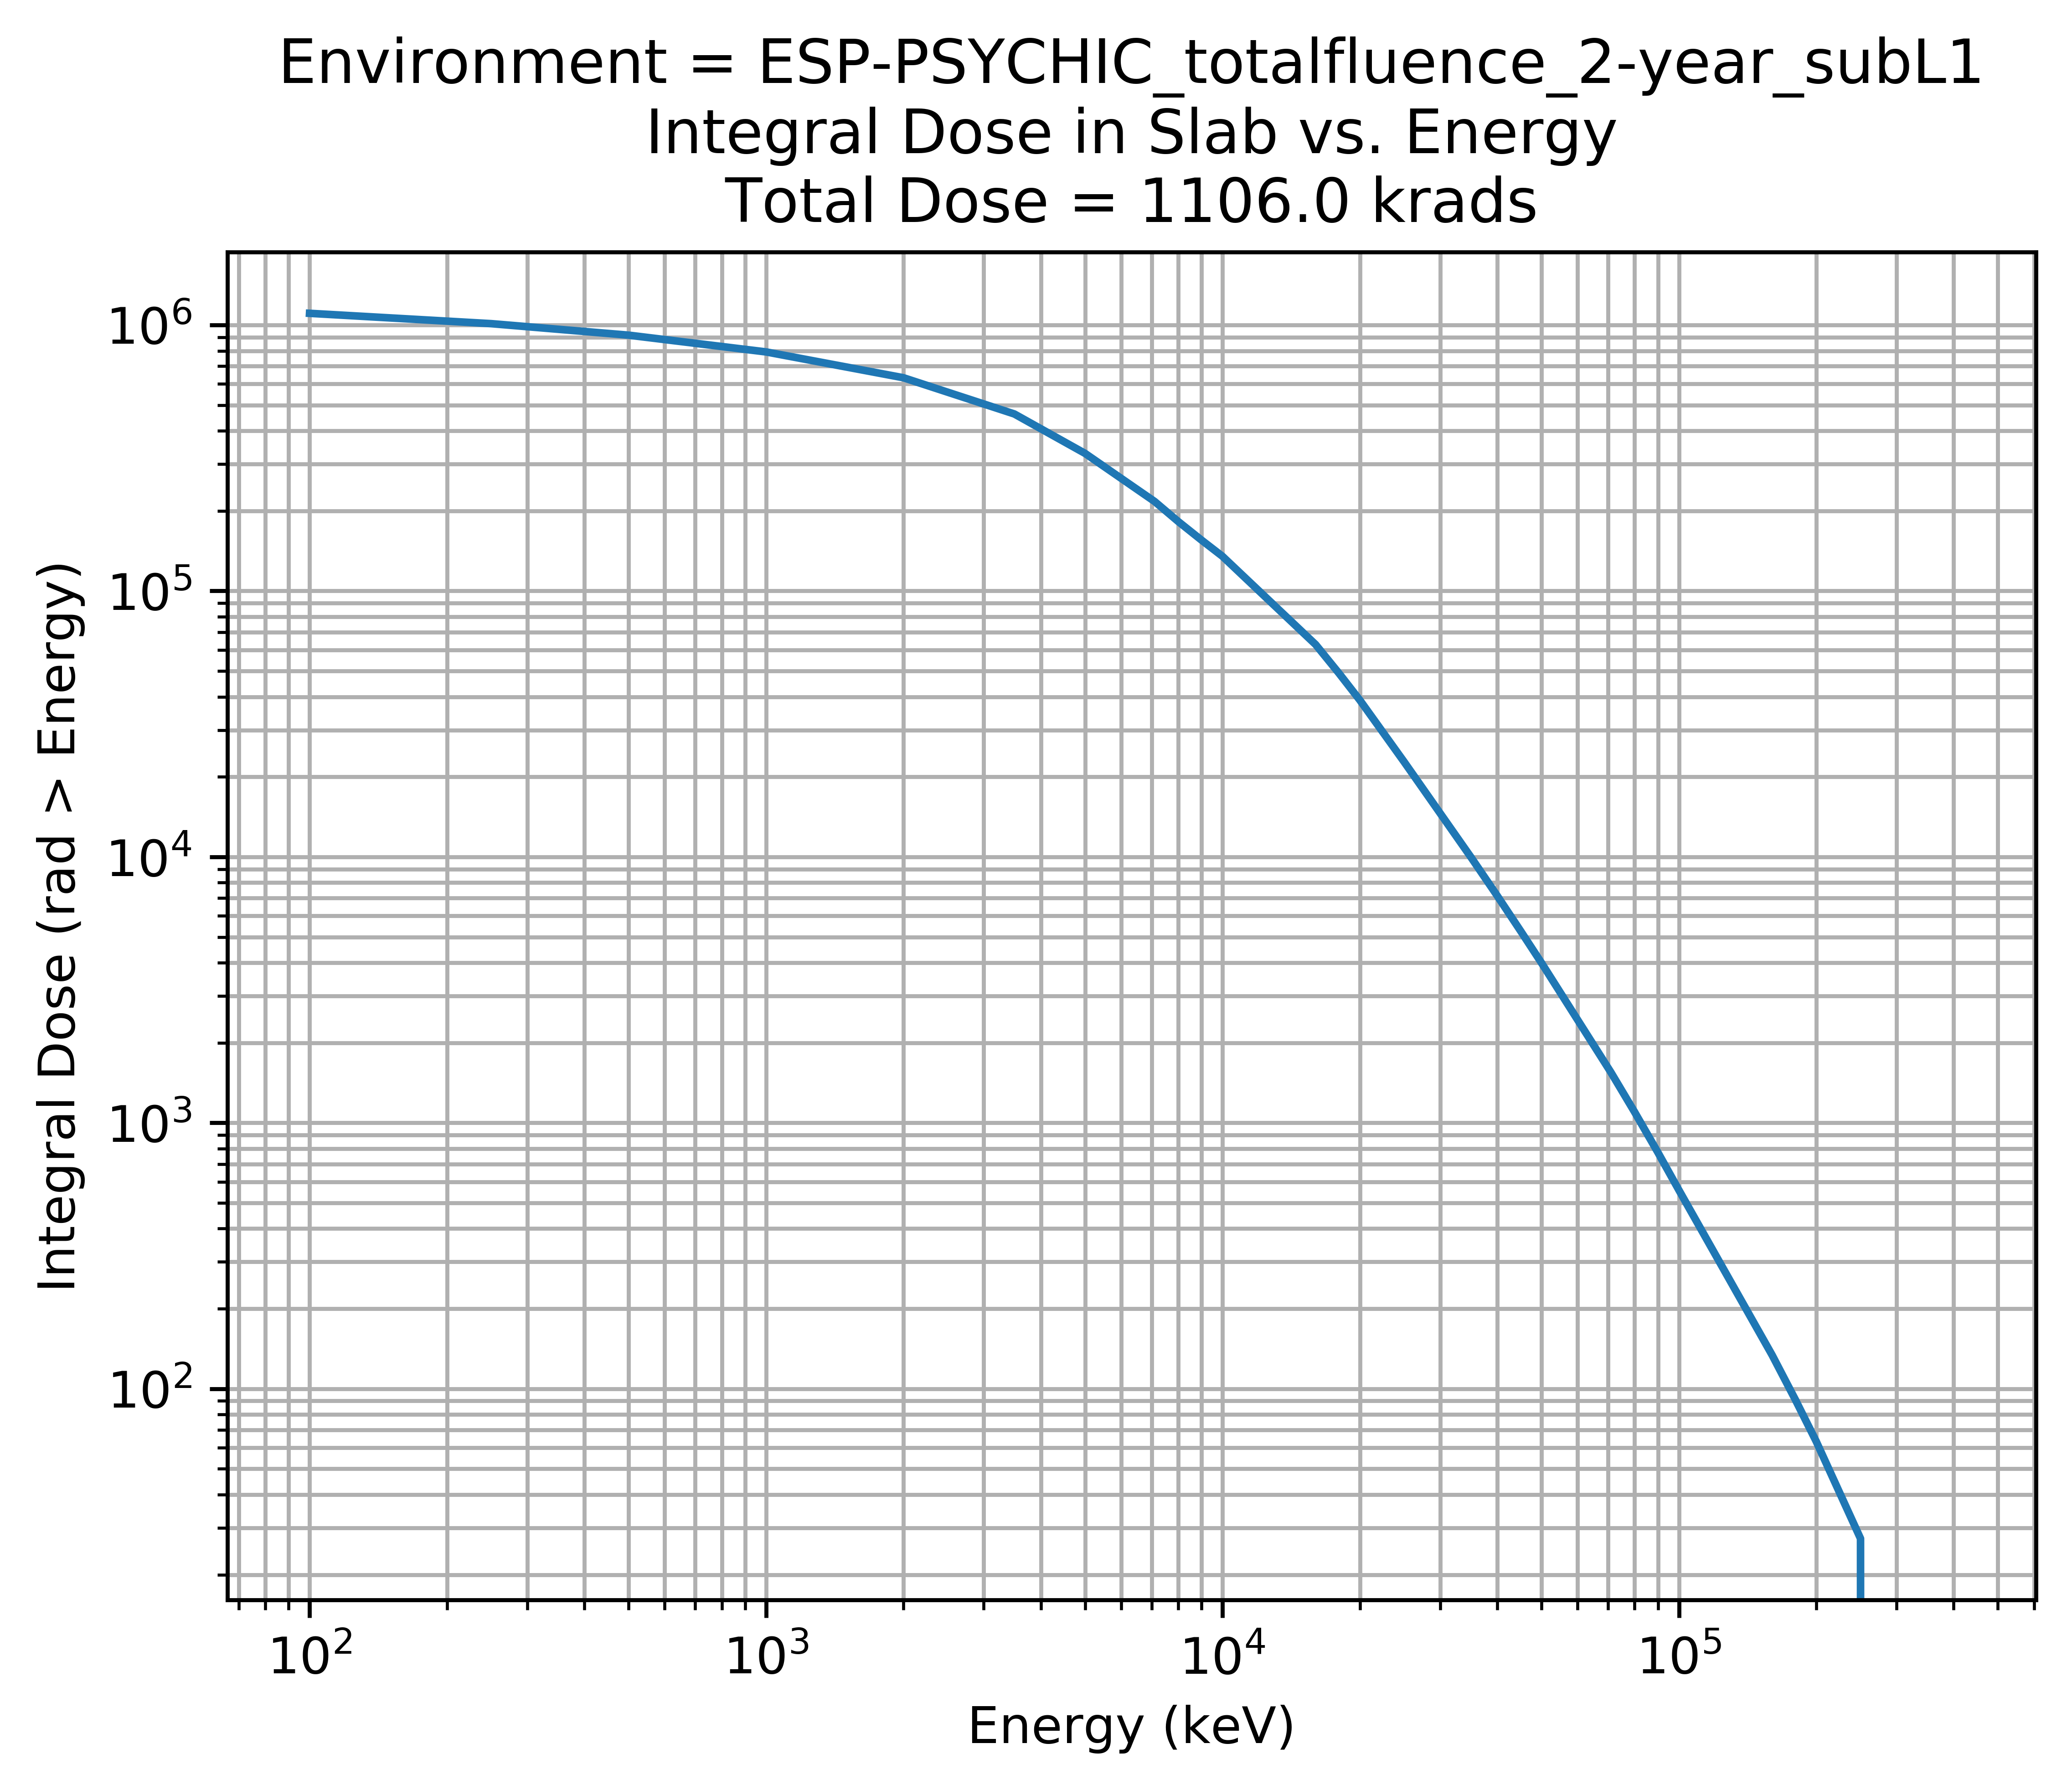
\includegraphics[width=0.95\textwidth]{../ESP-PSYCHIC_totalfluence_2-year_subL1_Integral_Dose_vs_Energy.png}
	\caption{The integral TID (greater than a certain energy) vs.\ energy for a 2-year isotropic SPE environment at 0.984 AU in $150 \mu$m of Kapton.}\label{fig:ESP-PSYCHIC_totalfluence_2-year_subL1_Integral_Dose_vs_Energy}
\end{figure}

\clearpage % forces the figure to drop before this point

%%%%%%%%%%%%%%%%%%%%%%%%%%%%%%%%%%%%%%%%%%%%%%%%%%%%%%%%%%%%%%%%%%
%%%%%%%%%%%%%%%%%%%%%%%%%%%%%%%%%%%%%%%%%%%%%%%%%%%%%%%%%%%%%%%%%%
\subsection{Low-Energy Solar Wind}
\label{ssec:TID-Low-Energy Solar Wind}

The low-energy solar wind environment (from L2-CPE) used in computing the TID to $150 \mu$m of Kapton can be found in Table \ref{tab:p95_sunward_solarwind_IMP} (Section \ref{ssec:natenv-Low-Energy Solar Wind}).  Dose vs.\ depth is covered in Section \ref{sssec:TID-LowE-Dose vs Depth} and Dose vs.\ energy in Section \ref{sssec:TID-LowE-Dose vs Energy}.

\subsubsection{Total Ionizing Dose vs.\ Material Depth}
\label{sssec:TID-LowE-Dose vs Depth}

\begin{figure}[htbp!]
	\centering
	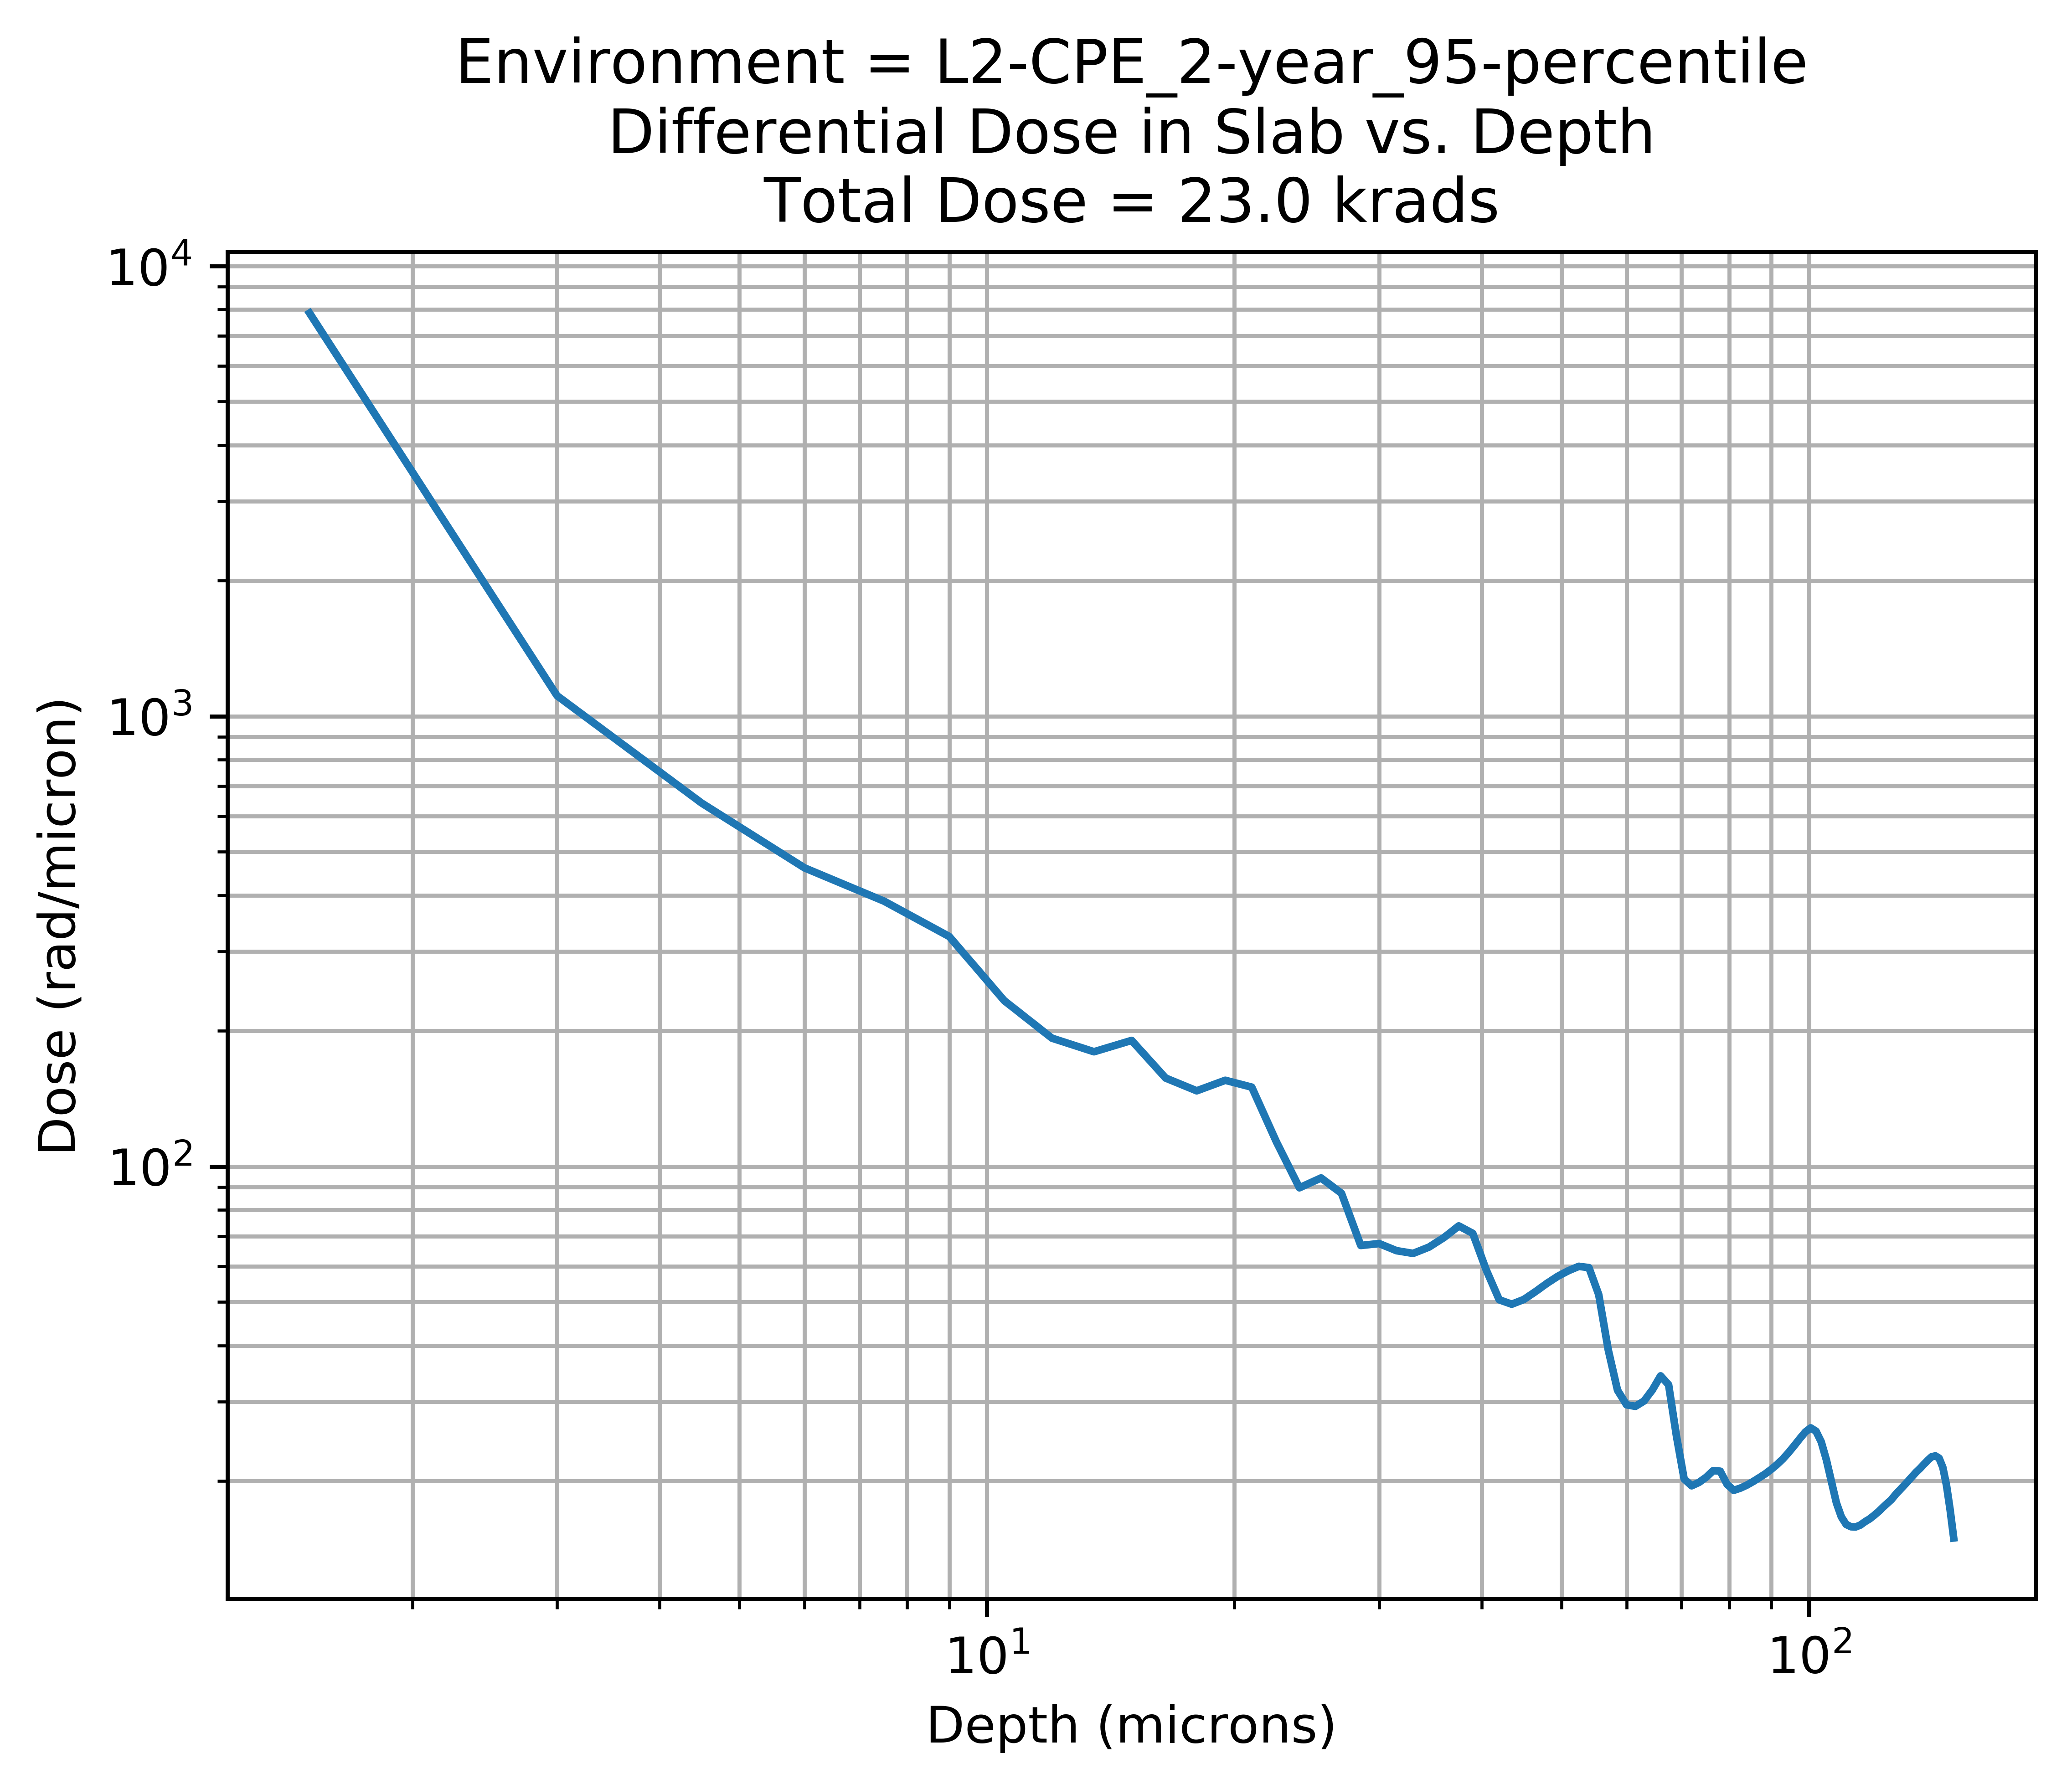
\includegraphics[width=0.95\textwidth]{../L2-CPE_2-year_95-percentile_Differential_Dose_vs_Depth.png}
	\caption{The differential TID vs.\ depth for a 2-year isotropic background solar wind environment at 1 AU in $150 \mu$m of Kapton.}\label{fig:L2-CPE_2-year_95-percentile_Differential_Dose_vs_Depth}
\end{figure}

\begin{figure}[htbp!]
	\centering
	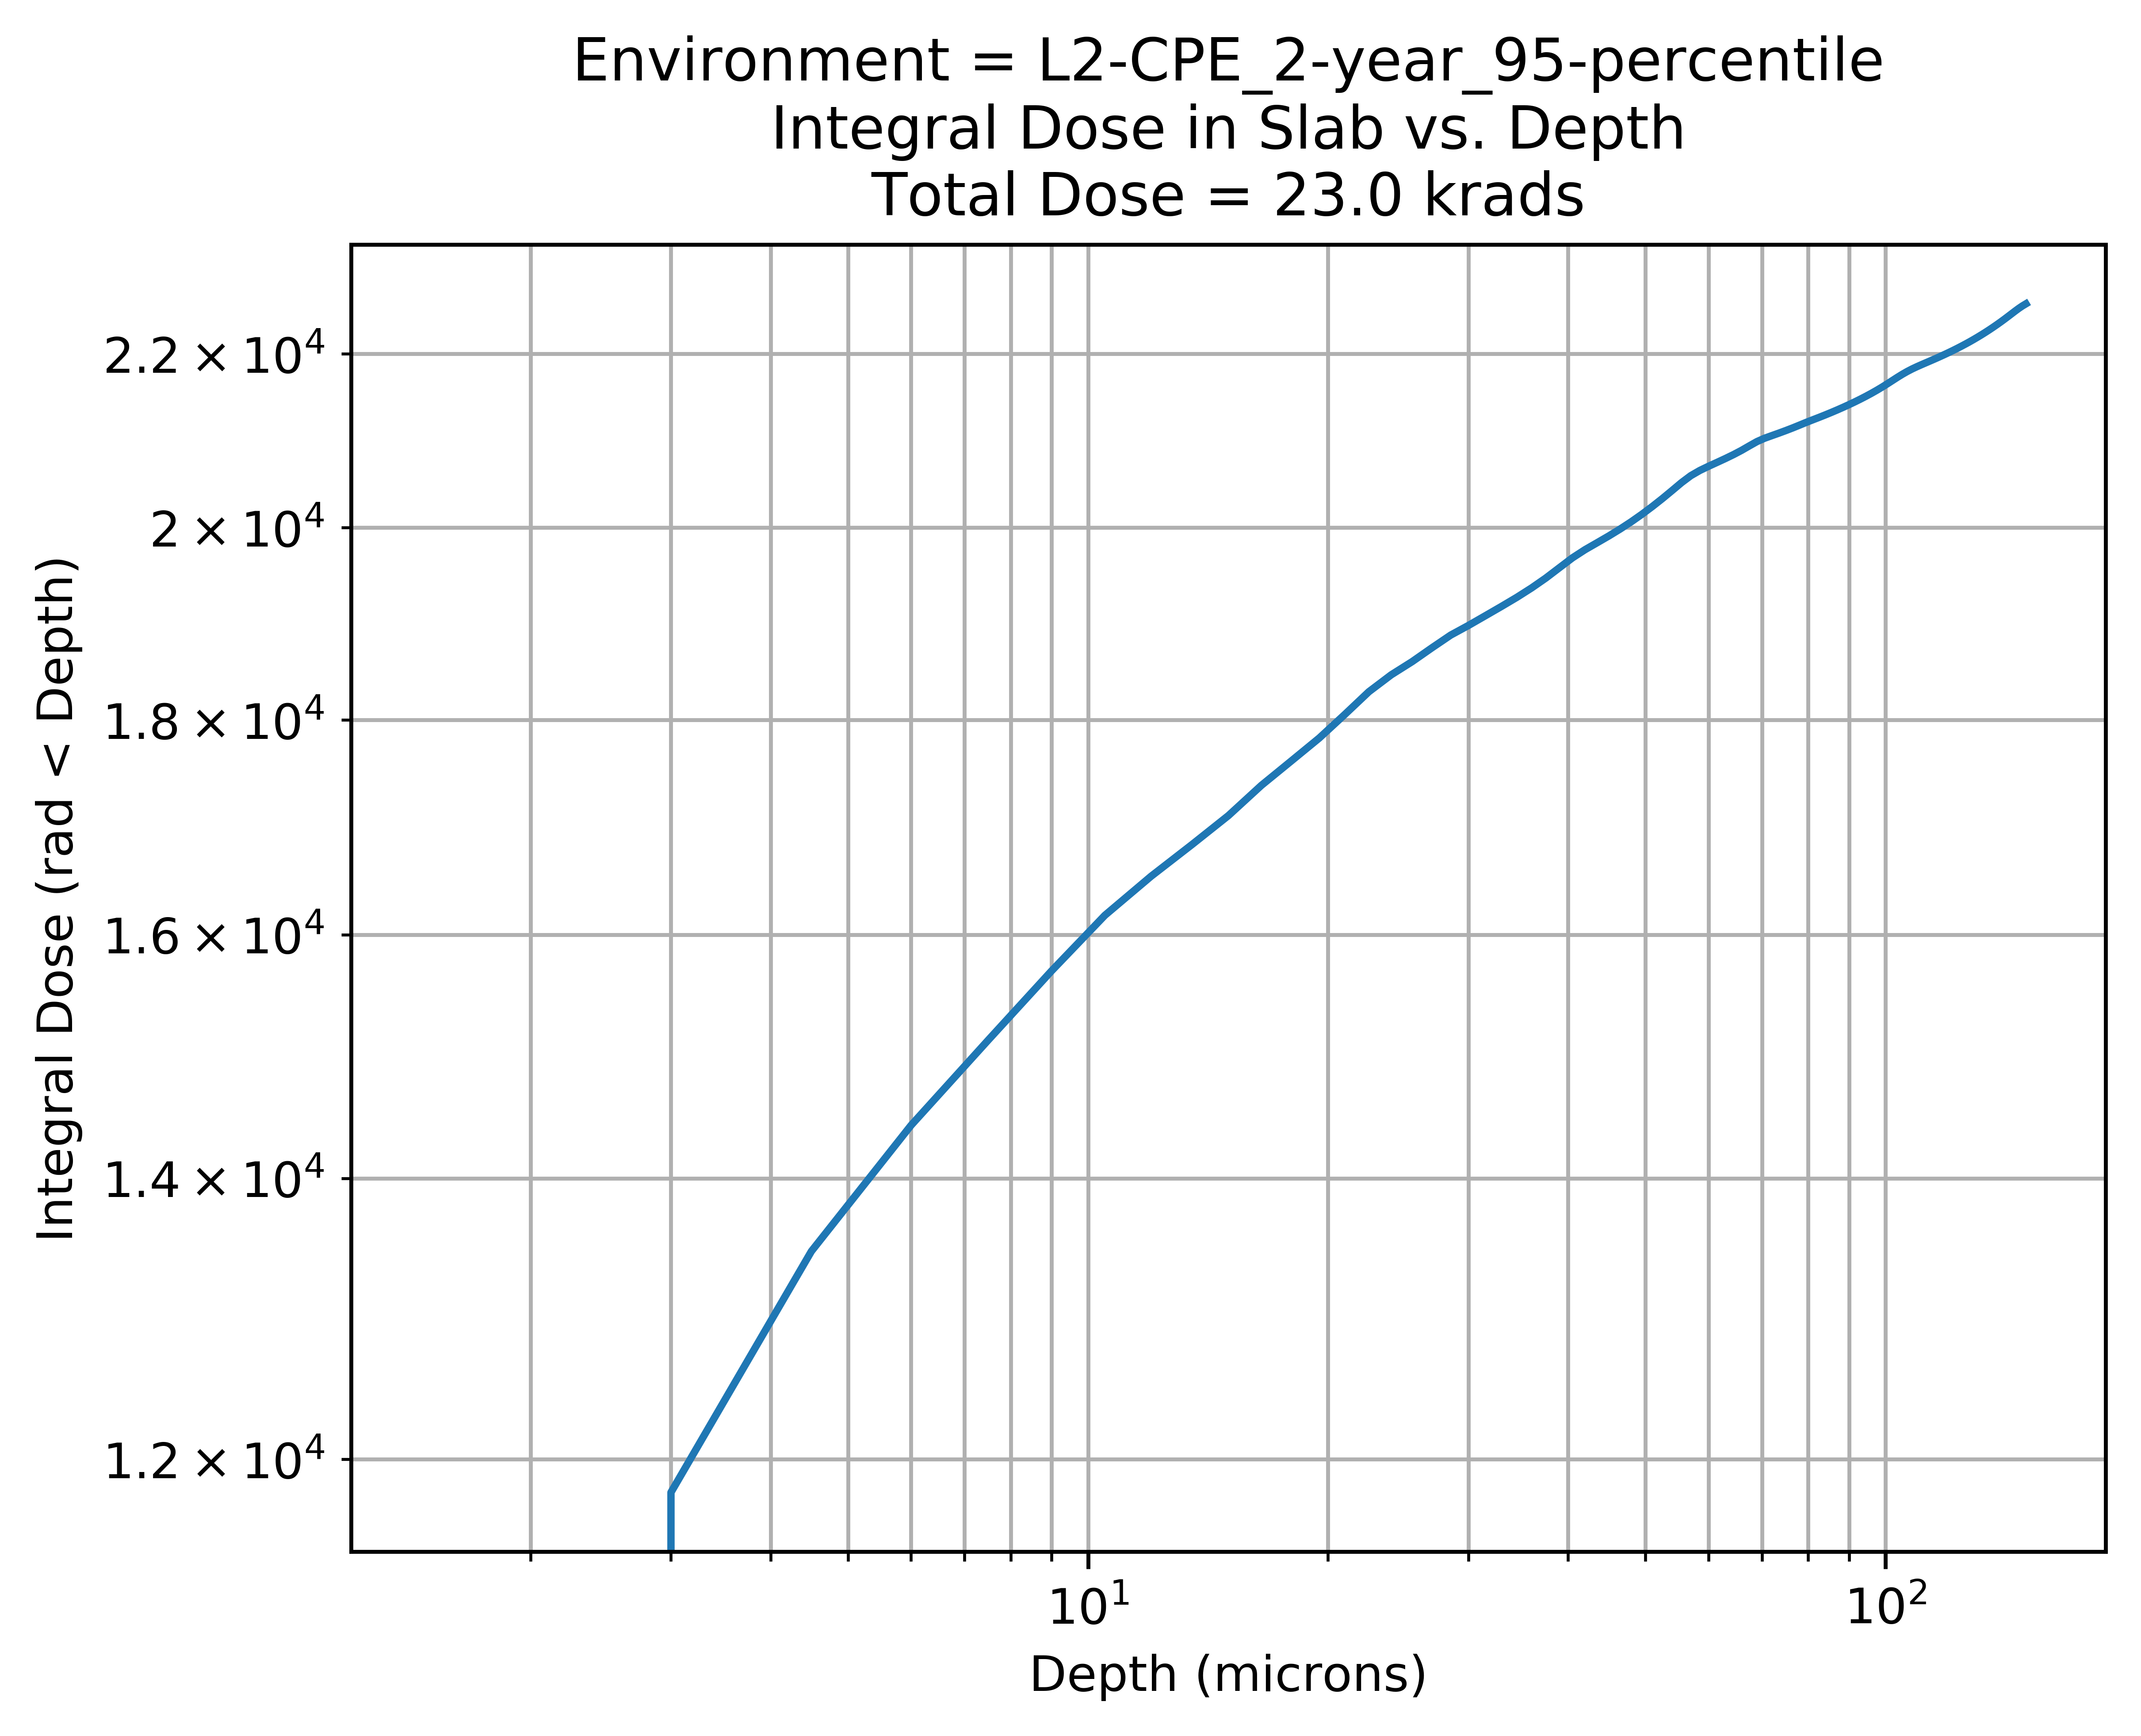
\includegraphics[width=0.95\textwidth]{../L2-CPE_2-year_95-percentile_Integral_Dose_vs_Depth.png}
	\caption{The integral TID (less than a certain depth) vs.\ depth for a 2-year isotropic background solar wind environment at 1 AU in $150 \mu$m of Kapton.}\label{fig:L2-CPE_2-year_95-percentile_Integral_Dose_vs_Depth}
\end{figure}

\clearpage % forces the figure to drop before this point


\subsubsection{Total Ionizing Dose vs.\ Proton Energy}
\label{sssec:TID-LowE-Dose vs Energy}

\begin{figure}[htbp!]
	\centering
	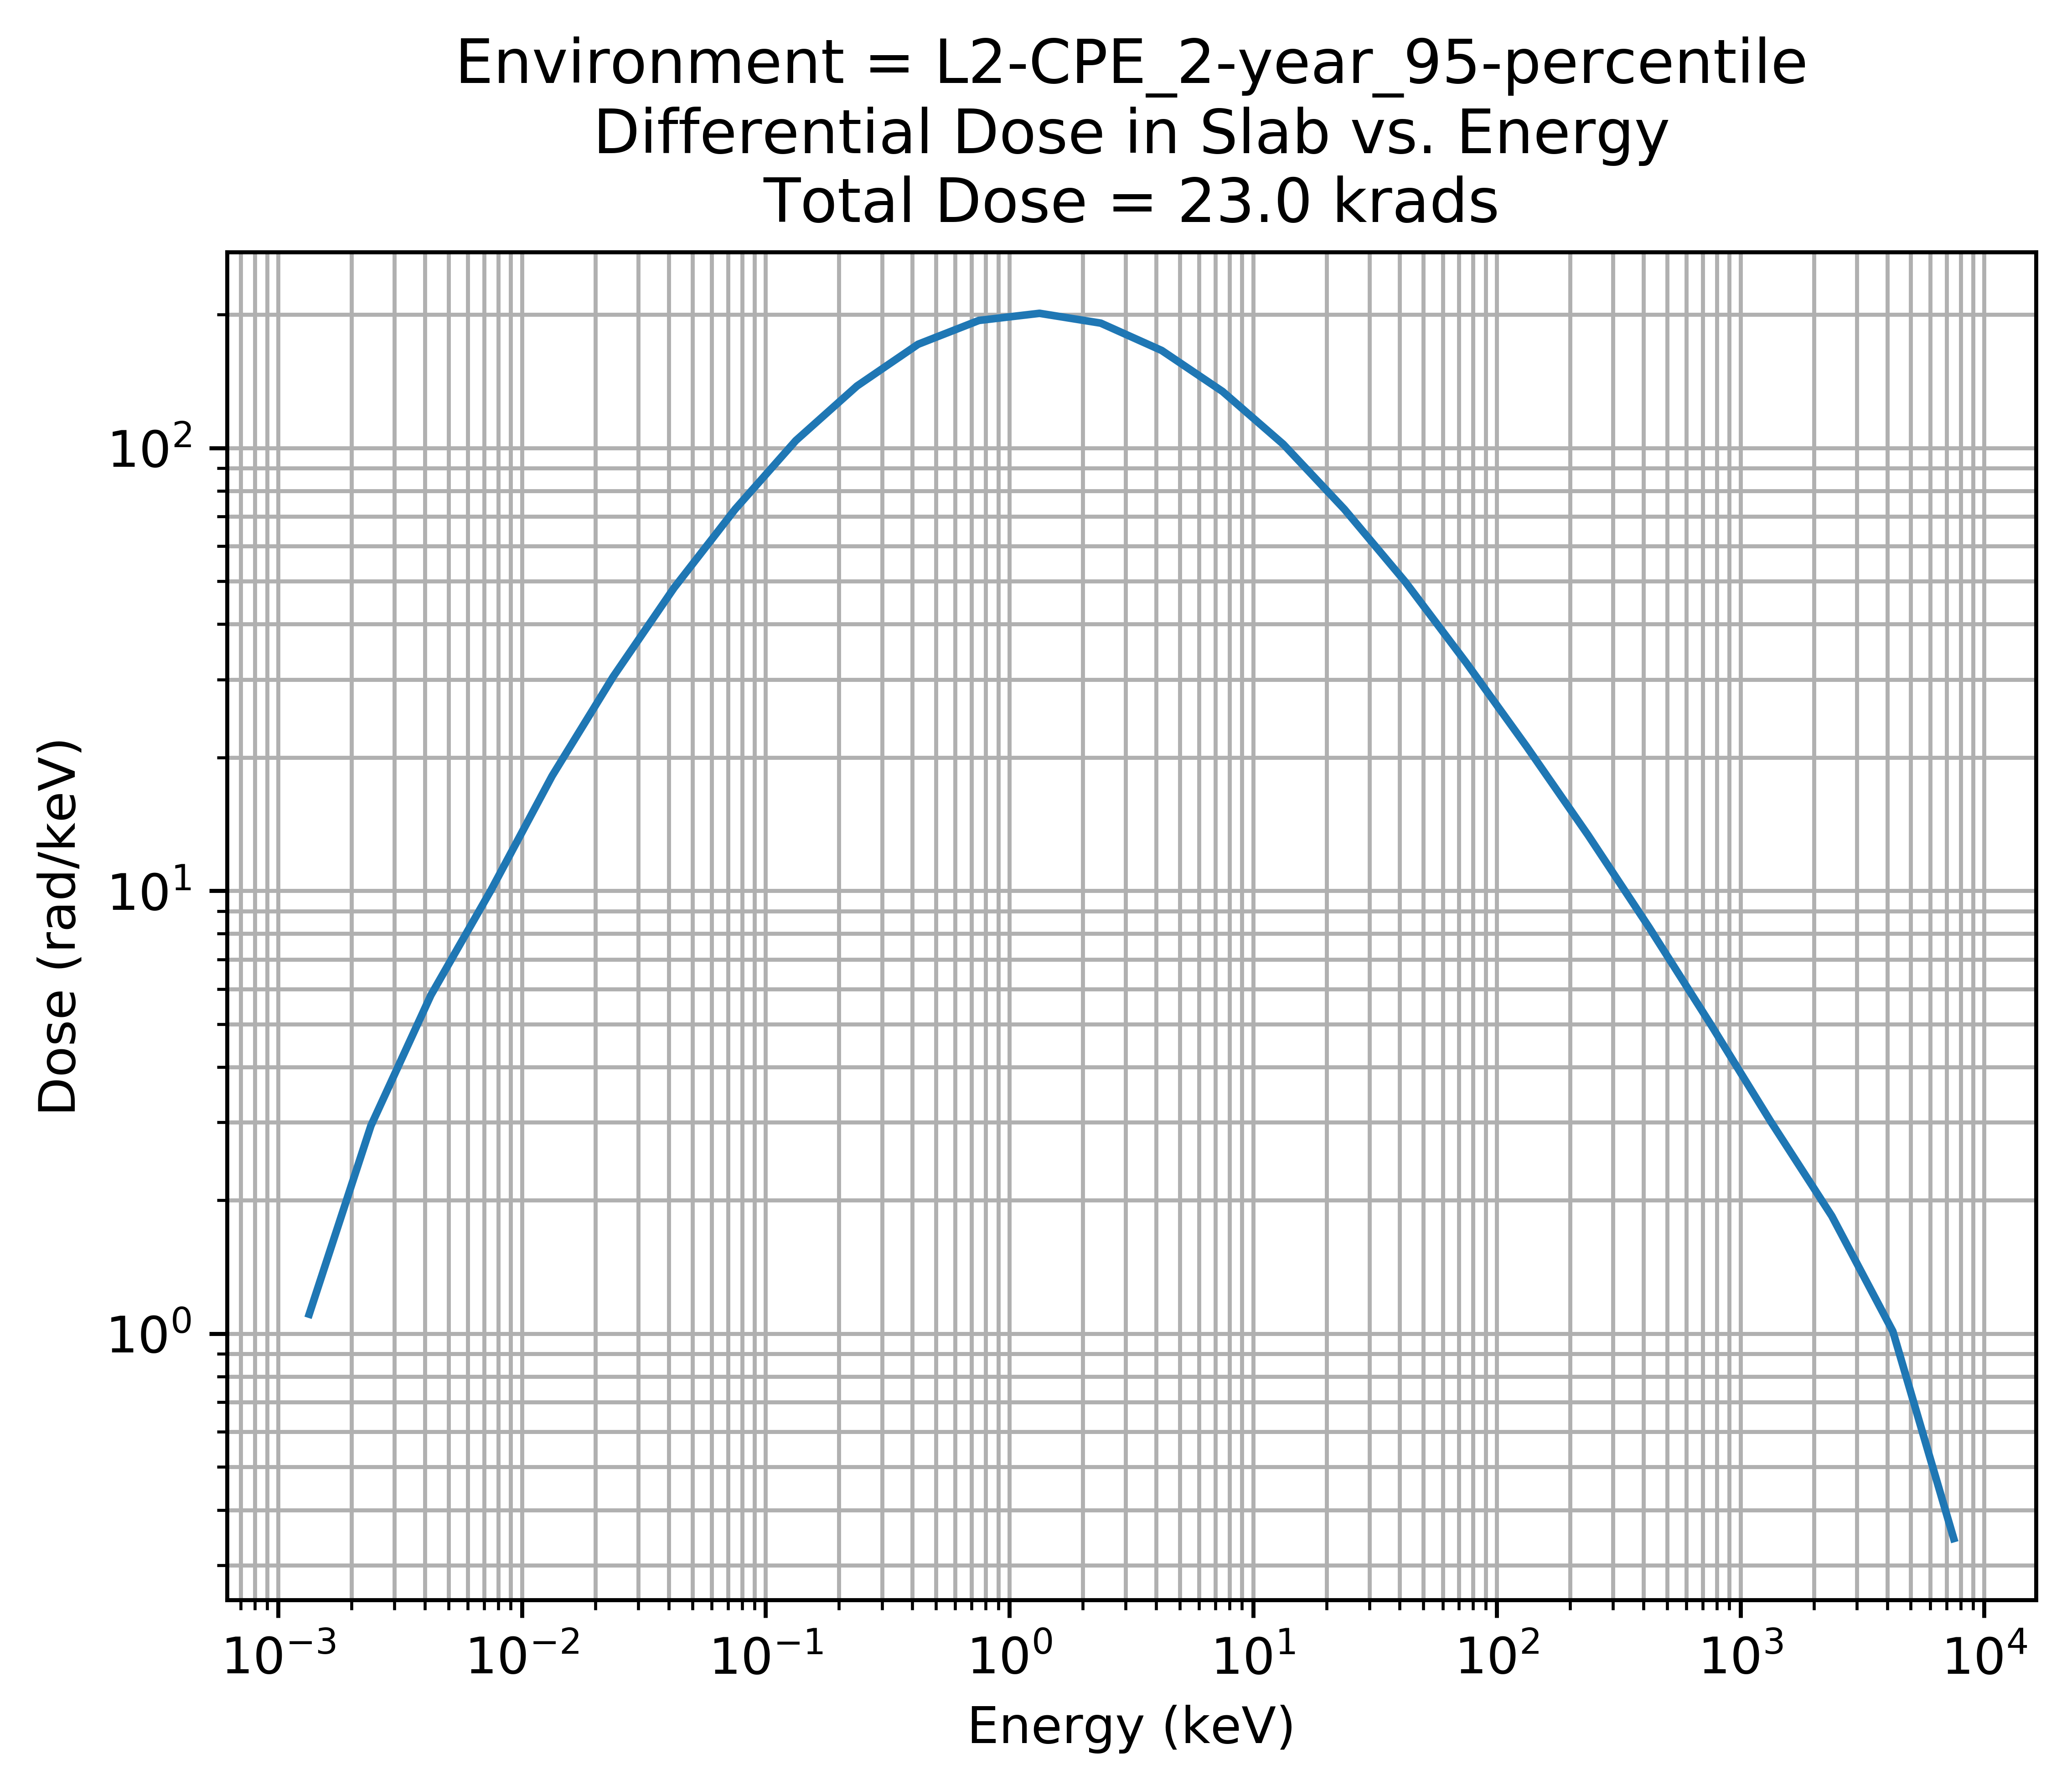
\includegraphics[width=0.95\textwidth]{../L2-CPE_2-year_95-percentile_Differential_Dose_vs_Energy.png}
	\caption{The differential TID vs.\ energy for a 2-year isotropic background solar wind environment at 1 AU in $150 \mu$m of Kapton.}\label{fig:L2-CPE_2-year_95-percentile_Differential_Dose_vs_Energy}
\end{figure}

\begin{figure}[htbp!]
	\centering
	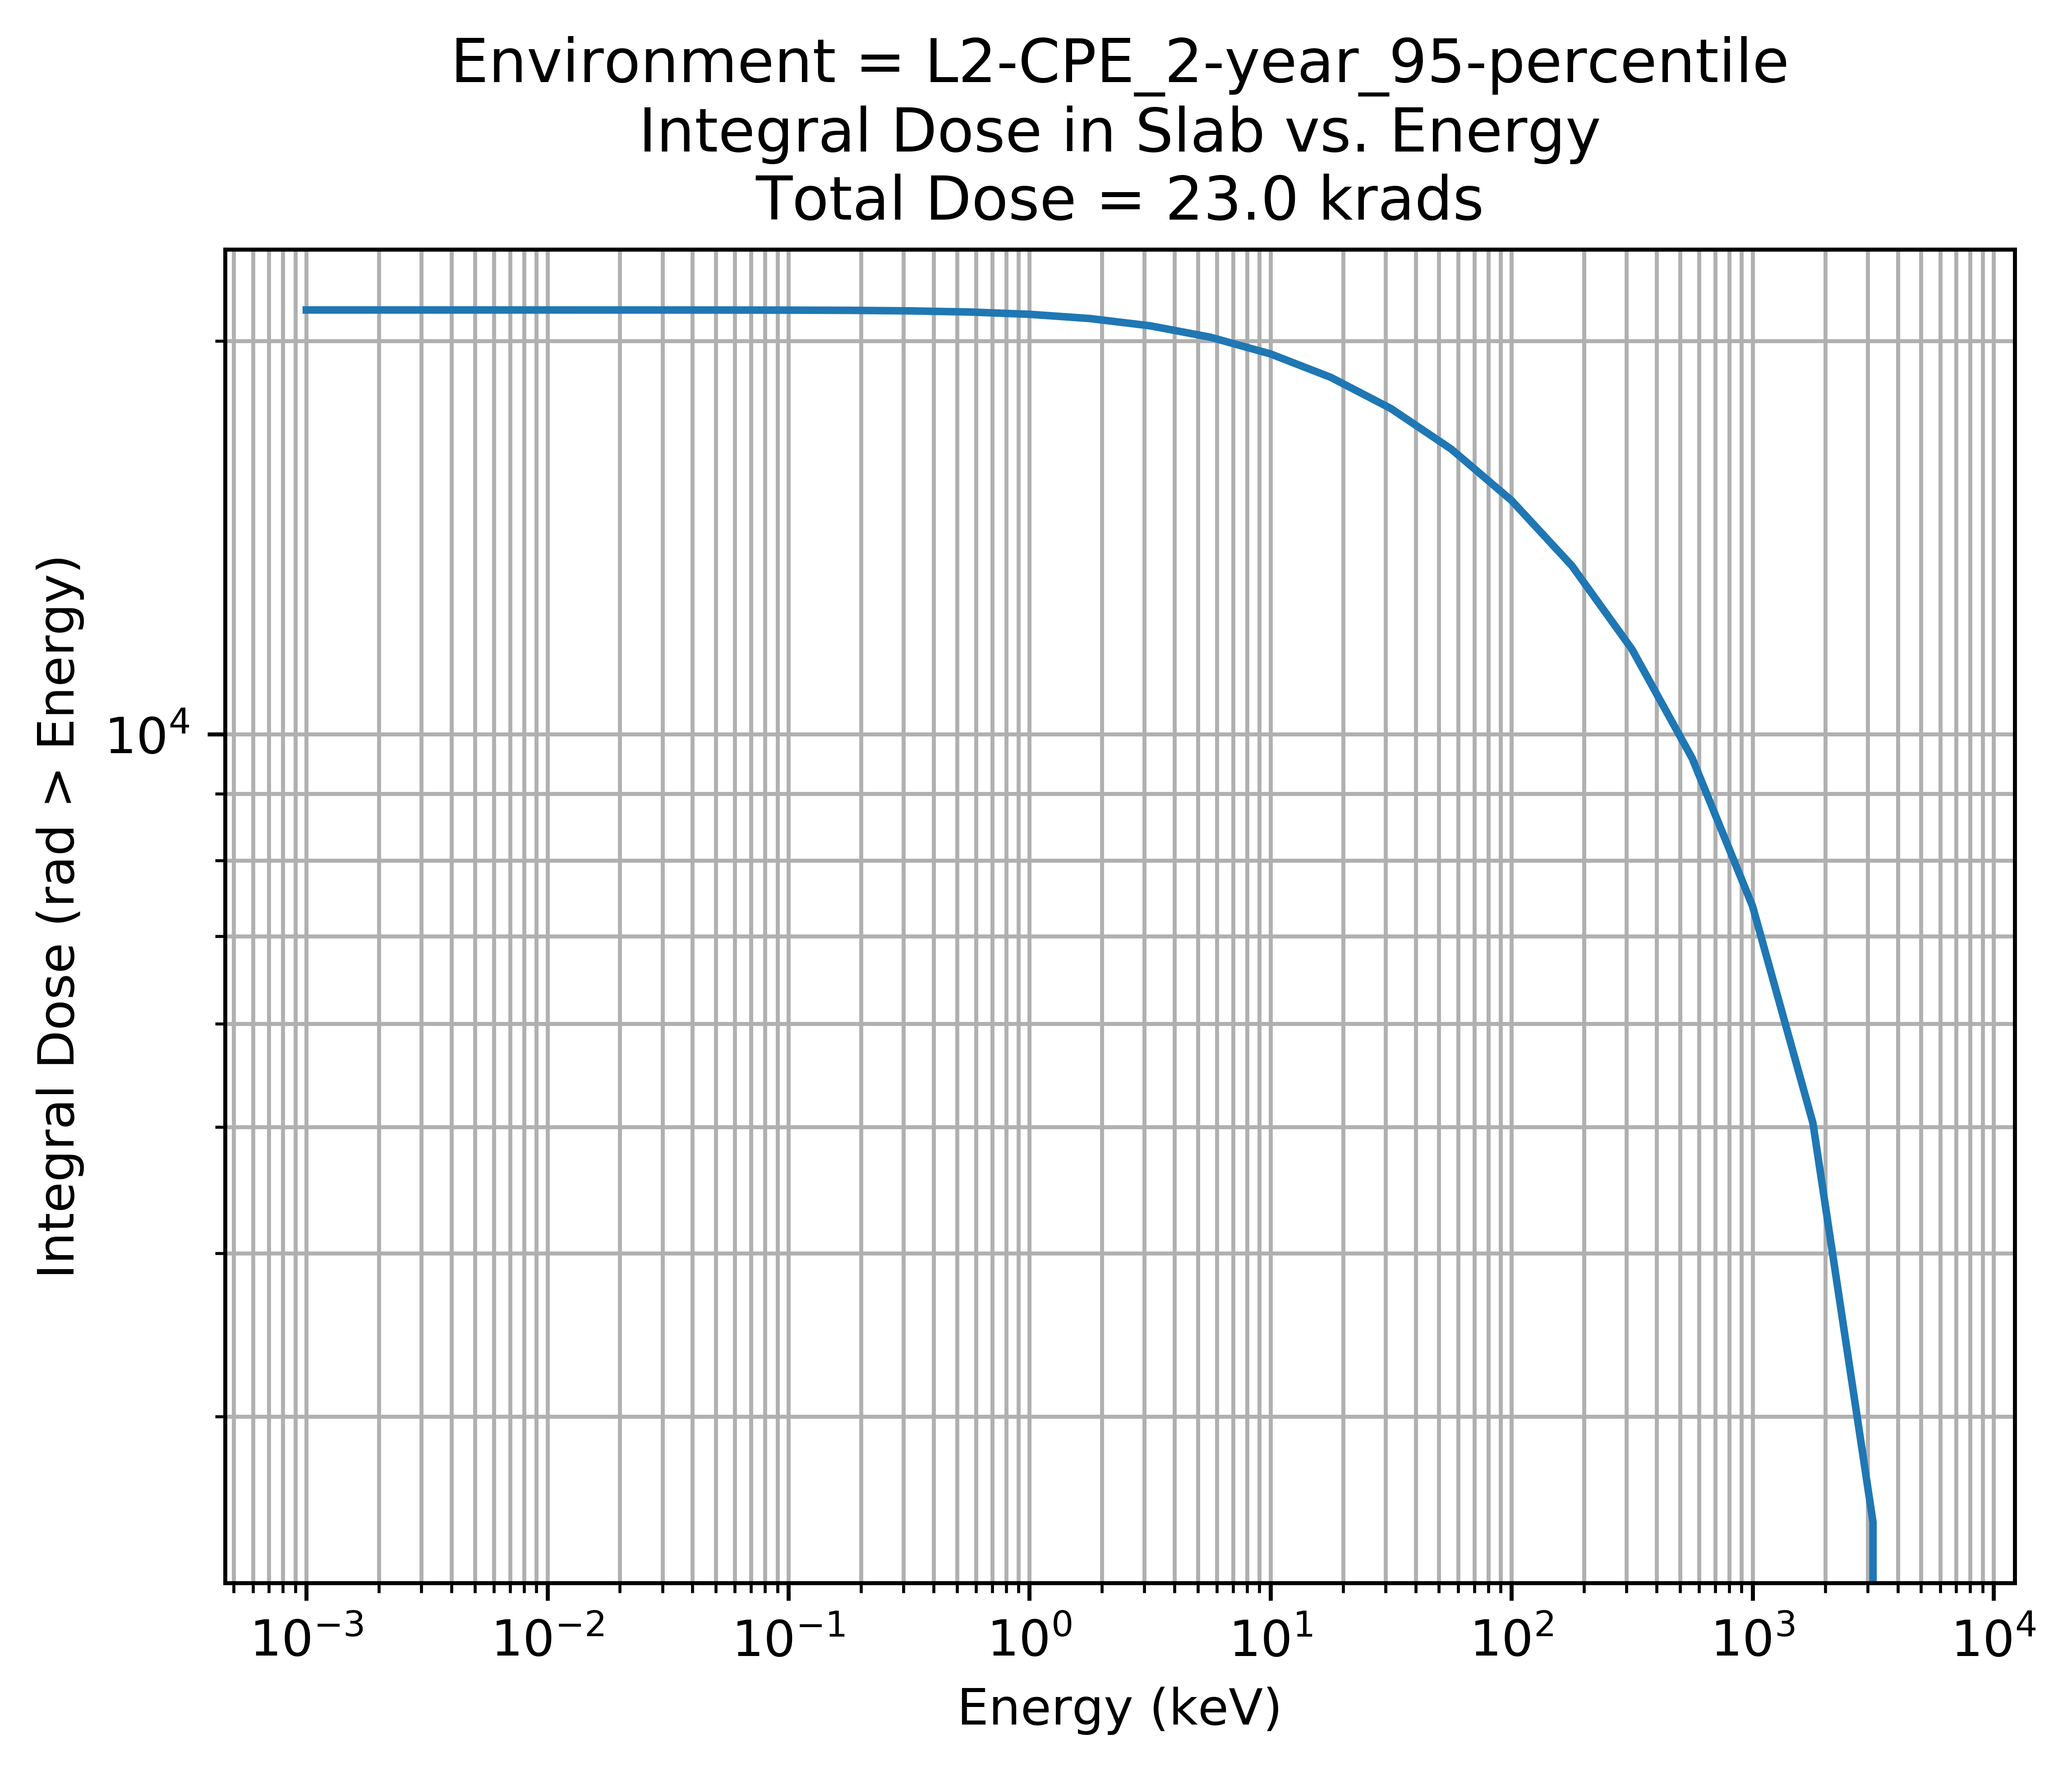
\includegraphics[width=0.95\textwidth]{../L2-CPE_2-year_95-percentile_Integral_Dose_vs_Energy.png}
	\caption{The integral TID (greater than a certain energy) vs.\ energy for a 2-year isotropic background solar wind environment at 1 AU in $150 \mu$m of Kapton}\label{fig:L2-CPE_2-year_95-percentile_Integral_Dose_vs_Energy}
\end{figure}

\clearpage % forces the figure to drop before this point

%%%%%%%%%%%%%%%%%%%%%%%%%%%%%%%%%%%%%%%%%%%%%%%%%%%%%%%%%%%%%%%%%%
%%%%%%%%%%%%%%%%%%%%%%%%%%%%%%%%%%%%%%%%%%%%%%%%%%%%%%%%%%%%%%%%%%
\section{Results}

The overall total ionizing dose (TID) in $150\mu$m of Kapton (as defined in Section \ref{sec:Materials}) from both the solar particle events (SPEs) (Section \ref{ssec:natenv-Solar Particle Events}) and the background solar wind (Section \ref{ssec:natenv-Low-Energy Solar Wind}) for 2 years in interplanetary space comes to \textbf{1.129 Mrads}. The driving factor is the SPE environment, which is assumed to be at solar maximum at a confidence level of $95\%$. The TID due to both heavy ions and electrons is omitted in this study.

Before the low-energy background solar wind was analyzed, it was unclear whether it would be a driver or not. Due to the thin layer of Kapton, it was expected only the mid- to low-energy component (i.e., $< 13.1$ MeV) would contribute to the TID. However, the results show that the background solar wind component provides only $2\%$ of the overall TID.

According to Figure \ref{fig:ESP-PSYCHIC_totalfluence_2-year_subL1_Integral_Dose_vs_Depth} for the SPE environment, roughly $25\%$ of the overall TID occurs in the first $3\mu$m of the kapton material, whereas for the background solar wind, Figure \ref{fig:L2-CPE_2-year_95-percentile_Integral_Dose_vs_Depth} shows that roughly $50\%$ of the overall TID occurs in the first $3\mu$m. This is consistent with the fact that the SPE environment has more higher energy protons than the background solar wind environment, and therefore will penetrate further into the kapton material. Given that a majority of the dose is deposited in the outermost layer of kapton, any thin film over the RCD might protect the inner layers from TID, especially due to the background solar wind. 
\newpage
\appendix

\section{Dose Percentile-Depth vs. Energy Parameters Fits}
\label{App:Dose Percentile-Depth vs. Energy Parameters Fits}

\begin{table}[!h]\centering
	\caption{Parameter fits to Equation \eqref{eq:double-power-law} for various dose percentiles using normally incident protons.}\label{tab:double-power-law-parameters}
	\begin{tabular}{|c | c | c | c | c |}\hline
		Percentile/100 & $a$ & $b$ & $c$ & $d$ \\\hline

0.05&8.445E+00&6.539E-01&4.543E+03&1.785E+00\\\hline
0.10&4.414E+00&6.654E-01&3.267E+03&1.786E+00\\\hline
0.15&2.923E+00&6.729E-01&2.682E+03&1.787E+00\\\hline
0.20&2.171E+00&6.793E-01&2.339E+03&1.788E+00\\\hline
0.25&1.723E+00&6.845E-01&2.109E+03&1.789E+00\\\hline
0.30&1.429E+00&6.894E-01&1.947E+03&1.790E+00\\\hline
0.35&1.216E+00&6.937E-01&1.826E+03&1.792E+00\\\hline
0.40&1.057E+00&6.976E-01&1.732E+03&1.793E+00\\\hline
0.45&9.332E-01&7.013E-01&1.658E+03&1.794E+00\\\hline
0.50&8.296E-01&7.043E-01&1.598E+03&1.795E+00\\\hline
0.55&7.407E-01&7.067E-01&1.549E+03&1.796E+00\\\hline
0.60&6.660E-01&7.089E-01&1.510E+03&1.798E+00\\\hline
0.65&6.006E-01&7.109E-01&1.479E+03&1.799E+00\\\hline
0.70&5.423E-01&7.128E-01&1.456E+03&1.800E+00\\\hline
0.75&4.868E-01&7.140E-01&1.438E+03&1.801E+00\\\hline
0.80&4.309E-01&7.141E-01&1.423E+03&1.802E+00\\\hline
0.85&3.744E-01&7.131E-01&1.412E+03&1.803E+00\\\hline
0.90&3.140E-01&7.104E-01&1.402E+03&1.804E+00\\\hline
0.95&2.441E-01&7.046E-01&1.396E+03&1.804E+00\\\hline
0.99&1.554E-01&6.904E-01&1.393E+03&1.805E+00\\\hline
0.999&9.998E-02&6.752E-01&1.394E+03&1.807E+00\\\hline
0.9999&7.282E-02&6.638E-01&1.385E+03&1.806E+00\\\hline

	\end{tabular}
\end{table}

\newpage
\section{Raw L2-CPE output of the Interplanetary Proton Environment}
\label{App:Raw L2-CPE output of the Interplanetary Proton Environment}

\lstinputlisting[language=xml,basicstyle=\footnotesize,frame=single,
caption={The sunward facing flux (worst-case) during solar maximum from IMP8 using L2-CPE.},label=lst:FLX_PTNXPOS_SWMX_IMP]{../L2CPE/FLX_PTNXPOS_SWMX_IMP.DAT}

%\section{References}
%\cleardoublepage
%\phantomsection
%\addcontentsline{toc}{section}{References}
%\bibliographystyle{agu}
%\bibliography{report}

\end{document}